%\documentclass[times, 10pt,twocolumn]{article}
%\documentclass[conference]{IEEEtran}
\documentclass[10pt, conference, compsocconf]{IEEEtran} 
%\usepackage{latex8}
%\usepackage{times}
\usepackage{url,hyperref}
\usepackage{subfigure}
\usepackage{tikz}
\usepackage{examplep}
\usepackage{moreverb}
\usepackage{algorithm}
\usepackage{boxedminipage}
\usepackage[noend]{algpseudocode}
\usepackage{listings}
\usepackage{amsmath,amsfonts,latexsym,graphicx}
\usepackage[tableposition=top,font=bf]{caption}
%\usepackage[tableposition=top,font=bf]{caption}

\lstset{language=C,numbers=left,basicstyle=\footnotesize,numberstyle=\footnotesize}
\usetikzlibrary{arrows,decorations.pathmorphing,backgrounds,fit,shapes.geometric}
\usepgflibrary{shapes.geometric}


%\documentclass[11pt]{article}
%\usepackage{fullpage}
%\usepackage{ijcai09}


%\setlength{\oddsidemargin}{0in}
%\setlength{\topmargin}{0in}
%\setlength{\textwidth}{6.5in}
%\setlength{\textheight}{8.5in}

\newtheorem{fact}{Fact}[section]
\newtheorem{lemma}{Lemma}[section]
\newtheorem{theorem}[lemma]{Theorem}
\newtheorem{assumption}[lemma]{Assumption}
\newtheorem{definition}[lemma]{Definition}
\newtheorem{corollary}[lemma]{Corollary}
\newtheorem{prop}[lemma]{Proposition}
\newtheorem{claim}[lemma]{Claim}
\newtheorem{remark}[lemma]{Remark}
\newtheorem{prob}{Problem}
\newtheorem{conjecture}{Conjecture}


\newenvironment{mylisting}
{\begin{list}{}{\setlength{\leftmargin}{1em}}\item\scriptsize}
{\end{list}}

\newenvironment{mytinylisting}
{\begin{list}{}{\setlength{\leftmargin}{1em}}\item\small\texttt}
{\end{list}}

\newenvironment{proof}{\vspace{-0.15in}\noindent{\bf Proof:}}%
        {\hspace*{\fill}$\Box$\par}
\newenvironment{proofsketch}{\noindent{\bf Proof Sketch.}}%
        {\hspace*{\fill}$\Box$\par\vspace{4mm}}
\newenvironment{proofof}[1]{\smallskip\noindent{\bf Proof of #1.}}%
        {\hspace*{\fill}$\Box$\par}

\newcommand{\etal}{{\em et al.}\ }
\newcommand{\assign}{\leftarrow}
\newcommand{\eps}{\epsilon}
%\documentstyle[times,art10,twocolumn,latex8]{article}

%------------------------------------------------------------------------- 
% take the % away on next line to produce the final camera-ready version 
\pagestyle{empty}

%------------------------------------------------------------------------- 
\begin{document}

\title{Parallel Information Set Generation for Kriegspiel 
       }
\title{Parallelizing  Information Set Generation for Game Tree Search Applications} 

\author{
\IEEEauthorblockN{Mark Richards, Abhishek Gupta, Osman Sarood and Laxmikant V. Kal\'e\\}
\IEEEauthorblockA{University of Illinois at Urbana-Champaign\\
Urbana, IL 61801, USA\\
(mdrichar, gupta59, sarood1, kale)@illinois.edu\\}
% For a paper whose authors are all at the same institution, 
% omit the following lines up until the closing ``}''.
% Additional authors and addresses can be added with ``\and'', 
% just like the second author.
%\and
%Second Author\\
%Institution2\\
%First line of institution2 address\\ Second line of institution2 address\\ 
%SecondAuthor@institution2.com\\
}

\maketitle
\thispagestyle{empty}

%\newtheorem{lemma}{Lemma}
%\newtheorem{theorem}[lemma]{Theorem}
%\begin{document}

%\title{Information Set Generation in Kriegspiel}
%\author{Abhishek Gupta\qquad Mark Richards\qquad Osman Sarood\\University of Illinois at Urbana-Champaign\\CS598LVK:
%Parallel Combinatorial Search} \maketitle

\begin{abstract}
Information Set Generation (ISG) is the identification of the set of paths in an
imperfect information game tree that are consistent with a player's
observations.  The ability to reason about the possible game history is
critical to the performance of game-playing agents.  ISG represents a class of
combinatorial search problems which is computationally intensive but challenging
to efficiently parallelize.

In this paper, we address the parallelization of information set generation in
the context of Kriegspiel (partially observable chess).  We implement the
algorithm on top of a general purpose combinatorial search engine and discuss
its performance using datasets from real game instances in addition to benchmarks. Further, we demonstrate the effect of load balancing strategies, problem sizes and computational granularity (grainsize parameters) on performance.  We achieve speedups of over 500 on 1,024 processors, far
exceeding previous scalability results for game tree search applications.
\end{abstract}

\section{Introduction}
In imperfect information games, players do not have access to full knowledge of
the world. Examples of imperfect information include hidden cards in
Poker~\cite{billings02challenge} or Bridge~\cite{ginsberg96partition}, hidden
tiles in Scrabble~\cite{richards07opponent}, or hidden pieces in 
Kriegspiel (partially observable chess)~\cite{li94chess}. The game tree nodes
which are indistinguishable to a player since they differ only in the
information that is hidden to the player by rule compose that player's {\em
information set.}  The ability to estimate the value of the possible states and
to reason about the probability distribution over those states is crucial to
playing imperfect information games well~\cite{schofield12hyperplay}. 

Information Set Generation (ISG) is an operation that game tree search agents
can use to identify nodes in the game tree that are consistent with their
observations~\cite{richards12information}.  Since the operation is
computationally intensive and may be repeatedly applied by a decision-making
agent, its efficiency is a key factor in an agent's overall performance.   

The term {\em belief state} is sometimes used interchangeably with information
set to refer to a probability distribution over possible worlds.  The latter
term comes from the game theory community and is preferred here.  A node in a
game tree denotes not only the current state of the game, but also uniquely
defines a path from the initial state or root node.  Hence, a game tree node
implicitly encodes not only the current state of the game but also the complete
history of all decisions made by all players up to that point in the game,
including the outcome of any chance moves such as dice rolls or card shuffling.
Knowing one's information set means knowing all possible game histories.

For many specific games, solving the information set generation problem is
trivial.  For example, in a Poker game, the unseen cards held by a player's
opponents may be any permutation of the cards not seen by that player (i.e.,
hole cards and any revealed community cards).  After the betting rounds, it
would not be reasonable to assume that each of these permutations of unseen
cards is equally probable, as betting decisions made by the players up to that
point would be affected by the quality of those players' cards.  However, the set of
{\em possible} hands for all of the opponents is easy to conceive and
enumerate.

However, for many games (such as Kriegspiel), information set generation is much more complicated.
After the first move by the opponent, a player faces uncertainty about the
location of the opponent's pieces.  Unlike Poker, it is not possible to simply
permute all of the opponent's possible pieces over all of the squares not
occupied by the player's own pieces.  A configuration of pieces for the
opponent is only valid if it can be reached by a legal sequence of moves.  In
the general case, finding the nodes in an information set is a combinatorial
search problem.

In this work, we show that ISG for Kriegspiel can be efficiently parallelized.
The primary contributions of this work are the following:
\begin{itemize}
\item
 We describe an
approach to efficient parallelization of an application - information set generation,  which is not typical of
high performance computing and scientific domain, yet important because of its usefulness in the field of artificial intelligence.
\item
 We present scalability results for our
parallel implementation of an information set generation algorithm for the game
of Kriegspiel using problem instances from real games. We achieve results which are unprecedented in game tree search application. 
\item
We demonstrate
the effects of load balancing strategy and grainsize on the parallel performance of our implementation. 
\end{itemize}

The remainder of the paper is organized as follows.  In Section~\ref{Kriegspiel}, we review
necessary background material, including the rules of Kriegspiel. Next, in
Section~\ref{info}, we describe the nature of the information set generation
problem and the algorithm used.  In Section~\ref{ParSSSE}, we describe our
parallel implementation, including the {\sc Charm++} Parallel State Space
Search Engine (ParSSSE) platform.  We then provide our experimental results in
Section~\ref{Results} followed by comparison with previous results and some discussion in Section~\ref{discuss}.  Related work is discussed in Section~\ref{Related}.  We
conclude with a discussion of future work.


\section{Background}\label{Kriegspiel}
Information Set Generation is the process of identifying the nodes in an
imperfect information game tree that are consistent with a player's
observations~\cite{richards12information}. Here, we present our techniques and
results in the context of a particular game: Kriegspiel~\cite{li94chess}.
However, the techniques and framework presented in this paper are general and
can be applied to ISG in other imperfect information games.
%\subsection{Kriegspiel}

Kriegspiel, or partially observable chess,  was invented by Henry Michael
Temple in 1899.  Historically, the game has required three parties: two
competing players and one referee.  Today, players often compete over a
computer network, with the role of the referee being automated.  One player
sees and controls only the white pieces; the other, black.  The referee tracks
both sets of pieces.  Instead of openly declaring their moves, players secretly
communicate move requests to the referee.  The referee, who knows the location
of all pieces, assesses the legality of the move according to the standard
rules of chess.  

If the move is legal, the referee executes the move and announces that a
legal move has been made and that it is the other player's turn to move.  If
the move is illegal because it is blocked by an opponent's piece or would place
or leave the active player in check, the referee announces, ``No.''  The player
then continues, without penalty, to attempt moves until one finally succeeds.
If a player has no legal moves because of stalemate or checkmate, the referee
announces the game's result.

All declarations by the referee are made to both players.  In
particular, a player will hear and know if her opponent has attempted an
illegal move, and will thus know that her opponent's pieces are configured in
such a way as to allow at least one attemptable move that is blocked or would
leave him in check.  

The referee makes other announcements besides declaring move illegal, and there
are several variations of the game that differ only in the nature of these
announcements.  In our implementation, the referee announces when a player is
in check, when a piece has been captured, and whenever a pawn may capture an
opponent's piece.  In the case of a capture, the referee announces the square
in which the capture occurs but not the identity of the captured piece.

In general, any move that is legal in a regular chess match may be at least
attempted by a player in Kriegspiel.  And any Kriegspiel move that is
ultimately allowed by the referee would also be a legal move in chess.    

\begin{figure}
\begin{center}
\begin{verbatim}
1. d4 {(:)}
   a5 {(:)}
2. Bg5 {(:)}
   b6 {(:)}
3. Nc3 {(:Bd8)}
   c5 {(:)}
4. d5 {(:Bd8;Tc5)}
   Na6 {(:)}
5. d6 {(:)}
   f6 {(:Td6)}
6. e4 {(:)}
   fxg5 {(Xg5:Td6;Tg5)}
7. Bc4 {(:)}
   exd6 {(Xd6:Td6)}
8. Qd5 {(:)}
   Qc7 {(:)}
9. Qf7+ {(:)} 
   Kd8 {:g6,Kxf7,Ke7}
10. Qxf8++ {(1-0:)}
\end{verbatim}
\end{center}
\caption{Listing of a Kriegspiel game resulting in checkmate by white after 10 moves. The final, legal move for each player is shown followed by the list of moderator declarations and all moves that were attempted but disallowed before the legal move was accepted.}
\label{listing}
\vspace{-0.1in}
\end{figure}

%\SubSection{Example}
\begin{figure}[ht]
\centering
\begin{minipage}[b]{0.45\linewidth}
\centering
\includegraphics[width=0.7\textwidth]{images/9B.png}
\caption{Actual Position}
\label{fig:figure1}
\end{minipage}
\hspace{0.5cm}
\centering
\begin{minipage}[b]{0.45\linewidth}
\centering
\includegraphics[width=0.7\textwidth]{images/OneView.png}
\caption{White's view}
\label{fig:figure2}
\end{minipage}
\vspace{-0.2in}
\end{figure}


\section{Information Set Generation}
\label{info}
%\subsection{Information Set Generation}
The concept of information sets is perhaps best explained through an example. 
Figures~\ref{listing}, \ref{fig:figure1} and~\ref{fig:figure2} show a full game listing and the associated pictorial progression of an actual
Kriegspiel game~\cite{li94chess}.  We have adopted the notation used by Wolfe for Berkeley Kriegspiel~\cite{wolfe07exploiting}.  Each numbered entry shows one complete turn for both White and Black.  The actual move is shown
first followed by a list of referee announcements.  Capture announcements are prefixed with an X and give the location
of the captured piece.  Similarly, pawn try announcements are prefixed with T.  Attempted moves that were ultimately
declared illegal are shown in a list following the `:'.  

Figure~\ref{fig:figure1} shows the true state of the game after nine moves by
each player.  Figure~\ref{fig:figure2} shows White's perspective of the game at
that point. At move 9, Black attempts to block a
potential threat along the diagonal by moving a pawn to g6, then attempts to
escape or capture a threat at f7.  When both of these attempts fail, Black can
infer that his king is being threatened by a protected bishop or queen at f7.
The attempt to move to e7 is Black's way of finding out whether the threatening
piece is a queen or bishop.  When this move fails, black knows it is White's
queen and ultimately retreats to d8.  Note that the failed moves by White on
turns 3 and 4 are a result of being blocked by the pawn at e2.


The listing in Figure~\ref{listing} corresponds to the referee's view of the game and would be useful for
post-game analysis or commentary.  During the game, players would not have access to the full information.  The
transcript from White's perspective is shown in Figure~\ref{filteredlisting}.  Note that Black's actual moves have been
replaced with ``??'' and lists of Black's illegal moves have been replaced with the {\em number} of illegal attempted
moves.  For example, on move 9, Black attempted three illegal moves.
\begin{figure}
%\begin{minipage}[b]{0.35\linewidth}
%\centering
%\small
\begin{verbatim}
1. d4 {(:)}
   ?? {(:0)}
2. Bg5 {(:)}
   ?? {(:0)}
3. Nc3 {(:Bd8)}
   ??  {(:0)}
4. d5 {(:Bd8;Tc5)}
   ??  {(:0)}
5. d6 {(:)}
   ?? {(:0,Td6)}
6. e4 {(:)}
   fxg5 {(Xg5:Td6;Tg5)}
7. Bc4 {(:)}
   ?? {(Xd6:Td6)}
8. Qd5 {(:)}
   ?? {(:0)}
9. Qf7+ {(:)} 
   ?? {:0}
10. Qxf8++ {(1-0:)}
\end{verbatim}
%\end{verbatim}
%\end{minipage}
%\begin{minipage}[b]{0.25\linewidth}
%\small
%\centering
%\begin{verbatim}
%\end{minipage}
%\vspace{-0.1in}
\caption{Observations received by White over the course of the game.  White does not know Black's actual moves but hears moderator announcements related to captures, pawn tries, and the number of attempted moves by Black that fail.}
\label{filteredlisting}
\vspace{-0.2in}
\end{figure}

The listing of a sequence of moves from the perspective of one player lists all of that player's moves exactly and
includes the declarations from the referee.  We refer to such a list as a player's observations.  Given a list of
observations for a sequence of moves, an information set is the set of all possible {\em sequences of moves for both
players}, that are consistent with those observations.  In other words, any sequence of moves that would have generated
the same sequence of observations for Black is in Black's information set.  Figure~\ref{abbrevoutput} shows a portion of the
information set for Black after both player's have made five moves.  From this list of possibilities, Black can infer
that White must have a bishop at g5 and a pawn at d6.  There are 25 possible sequences of moves that are consistent with
Black's observations up to that point. 

%Table~\ref{bothtimes} shows the size of the information sets for each player for
%each move in the game and the amount of time to find the full set on a single processor.  Appendix B shows the full
%output of the program for the same point in the game (five moves for each player) and illustrates all of the possible
%positions in the belief state.

\begin{figure}
\begin{mytinylisting}
1. Pa2:a4 Pa7:a5 2. Pd2:d4 Pb7:b6 3. Bc1:g5 Pc7:c5 \\
4. Pd4:d5 Nb8:a6 5. Pd5:d6 Pf7:f6 \\
\\
1. Pd2:d3 Pa7:a5 2. Bc1:g5 Pb7:b6 3. Pd3:d4 Pc7:c5 \\
4. Pd4:d5 Nb8:a6 5. Pd5:d6 Pf7:f6 \\
\\
1. Pd2:d4 Pa7:a5 2. Pa2:a4 Pb7:b6 3. Bc1:g5 Pc7:c5 \\
4. Pd4:d5 Nb8:a6 5. Pd5:d6 Pf7:f6 \\

%1. Pd2:d4 Pa7:a5 2. Bc1:f4 Pb7:b6 3. Bf4:g5 Pc7:c5 4. Pd4:d5 Nb8:a6 5. Pd5:d6 Pf7:f6 \\
%1. Pd2:d4 Pa7:a5 2. Bc1:g5 Pb7:b6 3. Pa2:a3 Pc7:c5 4. Pd4:d5 Nb8:a6 5. Pd5:d6 Pf7:f6 \\
%1. Pd2:d4 Pa7:a5 2. Bc1:g5 Pb7:b6 3. Pa2:a4 Pc7:c5 4. Pd4:d5 Nb8:a6 5. Pd5:d6 Pf7:f6 \\
%1. Pd2:d4 Pa7:a5 2. Bc1:g5 Pb7:b6 3. Pb2:b3 Pc7:c5 4. Pd4:d5 Nb8:a6 5. Pd5:d6 Pf7:f6 \\
%1. Pd2:d4 Pa7:a5 2. Bc1:g5 Pb7:b6 3. Pc2:c3 Pc7:c5 4. Pd4:d5 Nb8:a6 5. Pd5:d6 Pf7:f6 \\
%1. Pd2:d4 Pa7:a5 2. Bc1:g5 Pb7:b6 3. Pe2:e3 Pc7:c5 4. Pd4:d5 Nb8:a6 5. Pd5:d6 Pf7:f6 \\
%1. Pd2:d4 Pa7:a5 2. Bc1:g5 Pb7:b6 3. Pe2:e4 Pc7:c5 4. Pd4:d5 Nb8:a6 5. Pd5:d6 Pf7:f6 \\
%1. Pd2:d4 Pa7:a5 2. Bc1:g5 Pb7:b6 3. Pf2:f3 Pc7:c5 4. Pd4:d5 Nb8:a6 5. Pd5:d6 Pf7:f6 \\
%1. Pd2:d4 Pa7:a5 2. Bc1:g5 Pb7:b6 3. Pf2:f4 Pc7:c5 4. Pd4:d5 Nb8:a6 5. Pd5:d6 Pf7:f6 \\
%1. Pd2:d4 Pa7:a5 2. Bc1:g5 Pb7:b6 3. Pg2:g3 Pc7:c5 4. Pd4:d5 Nb8:a6 5. Pd5:d6 Pf7:f6 \\
%1. Pd2:d4 Pa7:a5 2. Bc1:g5 Pb7:b6 3. Pg2:g4 Pc7:c5 4. Pd4:d5 Nb8:a6 5. Pd5:d6 Pf7:f6 \\
%1. Pd2:d4 Pa7:a5 2. Bc1:g5 Pb7:b6 3. Ph2:h3 Pc7:c5 4. Pd4:d5 Nb8:a6 5. Pd5:d6 Pf7:f6 \\
%1. Pd2:d4 Pa7:a5 2. Bc1:g5 Pb7:b6 3. Ph2:h4 Pc7:c5 4. Pd4:d5 Nb8:a6 5. Pd5:d6 Pf7:f6 \\
%1. Pd2:d4 Pa7:a5 2. Bc1:g5 Pb7:b6 3. Nb1:a3 Pc7:c5 4. Pd4:d5 Nb8:a6 5. Pd5:d6 Pf7:f6 \\
%1. Pd2:d4 Pa7:a5 2. Bc1:g5 Pb7:b6 3. Nb1:c3 Pc7:c5 4. Pd4:d5 Nb8:a6 5. Pd5:d6 Pf7:f6 \\
%1. Pd2:d4 Pa7:a5 2. Bc1:g5 Pb7:b6 3. Nb1:d2 Pc7:c5 4. Pd4:d5 Nb8:a6 5. Pd5:d6 Pf7:f6 \\
%1. Pd2:d4 Pa7:a5 2. Bc1:g5 Pb7:b6 3. Qd1:d2 Pc7:c5 4. Pd4:d5 Nb8:a6 5. Pd5:d6 Pf7:f6 \\
%1. Pd2:d4 Pa7:a5 2. Bc1:g5 Pb7:b6 3. Qd1:d3 Pc7:c5 4. Pd4:d5 Nb8:a6 5. Pd5:d6 Pf7:f6 \\
%1. Pd2:d4 Pa7:a5 2. Bc1:g5 Pb7:b6 3. Qd1:c1 Pc7:c5 4. Pd4:d5 Nb8:a6 5. Pd5:d6 Pf7:f6 \\
%1. Pd2:d4 Pa7:a5 2. Bc1:g5 Pb7:b6 3. Ke1:d2 Pc7:c5 4. Pd4:d5 Nb8:a6 5. Pd5:d6 Pf7:f6 \\
%1. Pd2:d4 Pa7:a5 2. Bc1:g5 Pb7:b6 3. Ng1:f3 Pc7:c5 4. Pd4:d5 Nb8:a6 5. Pd5:d6 Pf7:f6 \\
%1. Pd2:d4 Pa7:a5 2. Bc1:g5 Pb7:b6 3. Ng1:h3 Pc7:c5 4. Pd4:d5 Nb8:a6 5. Pd5:d6 Pf7:f6 \\
\end{mytinylisting}
\caption{Abbreviated output from example game.  Three of 25 sequences that are consistent with Black's observations after five moves by each player.  The 25 sequences (or the states that result from them) compose Black's information set at that point in the game. From this, Black can infer that there is definitely a white bishop at g5 and a white pawn at d6.}
\label{abbrevoutput}
\vspace{-0.1in}
\end{figure}

%\begin{table}
%\centering
%\begin{tabular}{rrrrr}
% & \multicolumn{2}{c}{\bf White} & \multicolumn{2}{c}{\bf Black} \\
%{\bf Ply} & {\bf Size} & {\bf Time} & {\bf Size} & {\bf Time} \\
%1 & 18 & 0.000 & 20 & .000 \\
%2 & 18 & 0.000 & 19 & .000 \\
%3 & 18 & 0.000 & 404 & .008\\
%4 & 279 & 0.008 & 401 & .024\\
%5 & 242 & 0.028 & 1472 & .044\\
%6 & 216 & 0.052 & 155 & .096\\
%7 & 176 & 0.064 & 293 & .116\\
%8 & 3406 & 0.092 & 158 & .128\\
%9 & 2191 & 0.288 & 118 & .148\\
%10 & 1423 & 0.508 & 25 & .152\\
%11 & 1363 & 0.596 & 798 & .164\\
%12 & 1416 & 0.744 & 518 & .192\\
%13 & 1416 & 0.836 & 13564 & .304\\
%14 & 3440 & 0.97 & 12394 & .776\\
%15 & 3428 & 1.25 & 343652 & 3.75\\
%16 & 50521 & 1.82 & 320704 & 17.3\\
%17 & 43192 & 5.91 & 490162 & 99.9\\
%18 & 26128 & 7.94 & 3792 & 119\\
%19 & 19061 & 9.92 & 14836 & 121\\
%\end{tabular}
%\caption{Solution counts and running times for a sample Kriegspiel game}
%\label{bothtimes}
%\end{table}

%Table~\ref{sampletimes}
%\begin{table}
%\begin{tabular}{ccc}
%1 & 20 & .000\\
%2 & 19 & .000\\
%3 & 404 & .008\\
%4 & 401 & .024\\
%5 & 1472 & .044\\
%6 & 155 & .096\\
%7 & 293 & .116\\
%8 & 158 & .128\\
%9 & 118 & .148\\
%10 & 25 & .152\\
%11 & 798 & .164\\
%12 & 518 & .192\\
%13 & 13564 & .304\\
%14 & 12394 & .776\\
%15 & 343652 & 3.75\\
%16 & 320704 & 17.3\\
%17 & 490162 & 99.9\\
%18 & 3792 & 119\\
%19 & 14836 & 121 \\
%\end{tabular}
%\caption{Solution counts and running times for a sample Kriegspiel game}
%\label{blacktimes}
%\end{table}

   
\textbf{The Information Set Generation}
(ISG) operation can be formulated as a combinatorial search problem.  The input to the algorithm is a list
of $t$ observations for one player $k$ (denoted $o_{1:t}^{(k)}$ in a Kriegspiel game.    
\begin{figure}[htpb]
\small
%\begin{algorithm}
\begin{boxedminipage}{\columnwidth}
\begin{algorithmic}[1]
\Function{DFS-Infoset}{$a_{1:t}$, $o_{1:T}^{(k)}$, $I$, $s$, $t$}
  \If {$t > T$}
    \State {$I \leftarrow I \cup a_{1:t}$} %\Comment{$a_{1:t}$ leads to $o_{1:T}$ for $P_k$; add it to the information set.}
  \Else {
    \For{\textbf{each} legal action $a$ at $s$}
      \State {$s'$ = {\sc GetNextState}($s$,$a$)}\label{line:update}
      \If {$s'.o_{t+1}^{(k)}=o_{t+1}^{(k)}$}
        \State {{\sc DFS-Infoset}($a_{1:t}a$, $o_{1:T}^{(k)}$, $I$, $s'$, $t+1$)} 
          %\Comment{ Recall that $N(a_{1:t}a) = T(T(a_{1:t}),a)$}
      \EndIf
    \EndFor
  }\EndIf
\EndFunction
\end{algorithmic}
\end{boxedminipage}
\caption{Core of Information Set Generation Algorithm}
\label{codelisting1}
\vspace{-0.2in}
\end{figure}


The nodes in the search tree at depth $n$ correspond to possible move 
sequences of $n$ plies from the start state.  (A sequence of $t$ actions from
the start state is denoted $a_{1:t}$.) There is a search space variable for
each ply in the game, and the values that a variable can take on are all
possible legal moves.  Information set generation, then, is an all-solutions
search through the space.  Whenever a node in the search tree is found to be
inconsistent with the actual observation given in the input, the subtree rooted
at that node is pruned (i.e., search is discontinued along that path).  There
are three types of observations that must match in order for a state $s$ to be
included in the information set $I$ at depth $t$: check status, pawn tries, and
illegal moves available/attempted.


Figure~\ref{codelisting1} shows the function at the heart of our information set generation algorithm.  The actual
observations can be viewed as global, read-only variables.  All solutions (i.e., all nodes in the information set) will
be located at the same depth in the tree: the depth that is equal to the number of plies in the observation list.
Referee announcements regarding pawn tries or a player being in check are made prior to a move.  The algorithm checks
for the consistency of these observations at line $7$.  If the search reaches the appropriate depth and passes these
tests, then a solution has been found and is added to the information set (line $3$).  

%Otherwise, we consider the possible moves that can be made from that state.  If the player whose turn it is to move at
%the current level of the search tree is the same player from whose perspective we have received observations, then the
%next step is to make sure that every legal move that was attempted at the player at that ply is also at least
%attemptable at the game position that corresponds to the game tree node (lines $15--22$).  We know exactly the legal
%move that was ultimately made at this depth (because we are assuming perfect recall), and we check to make sure that
%this move is indeed legal (pruning otherwise).  If so, we apply that move and recurse (lines $24--32$).  This
%corresponds to a ``forced move'' in the general search paradigm.
%
%On the other hand, if the player whose turn it is to move at the current depth of the search tree is the opponent, then
%must consider all possible legal moves to branch on.  We first check to make sure that the number of legal moves from
%this position is at least as large as the number of illegal moves that the opponent attempted (i.e., the number of times
%the referee said ``No'' before finally accepting the opponent's move).  This is shown in lines $39--42$.  At this point
%we generate a child for each move that would be accepted by the referee and recurse (lines $44--52$).
%
%One of our goals was to assess the varying utilities of the different pruning criteria.  We tried some different
%orderings of the tests and were somewhat surprised (and disappointed) to see that there was actually a fairly minimal
%impact on performance.  This could be due to the fact that because of the tedious nature of encoding problem instances
%from actual games, we were not able to run experiments of a wide variety of types of positions (i.e., different styles
%of play).

%\begin{figure}
%%\begin{listing}
%\begin{lstlisting}
%void generateInformationSet(uint16_t* trueState, uint16_t* possState, bool whiteMove, 
%	uint16_t* possHistory, uint16_t** levels, int depth)
%{
%  if (!samePawnTries(trueState, possState, whiteMove)) return;  
%  if (!sameCheckStatus(trueState, possState, whiteMove)) return; 
%  if (depth == maxdepth) { // Then we have found a solution
%	nSolutions++; return; // Report solution
%  }
%  uint16_t newPossState[16]; 
%  int nMoves = 0;
%  generateAttemptableMoves(possState, whiteMove, levels[depth], nMoves,false);
%  checkForCheck(possState, whiteMove, levels[depth], nMoves); // prunes if not equal
%  assert (nMoves < NMOVES); // 
%
%  if (whitePerspective == whiteMove) { // move from perspective player 
%    SetMove& failures = failedMoves[depth];
%    for (SetMove::const_iterator itr = failures.begin(); itr != failures.end(); ++itr) {
%      uint16_t move = *itr ;
%      if (!foundMatchingMove(move,levels[depth],nMoves)) {
%        return; // Prune: one of my own failed moves is not attemptable in this state
%      }
%    }
%    // We know exactly what the actual move was; make it
%    uint16_t& actualMove = moveHistory[depth];
%    if (!foundMatchingMove(actualMove,levels[depth],nMoves)) {
%      return; // Prune (because the move that we know we made at this depth is not legal)
%    }
%    // Otherwise, recurse 
%    applyMove(possState,newPossState,actualMove);
%    possHistory[depth] = actualMove;
%    generateInformationSet(newTrueState, newPossState, !whiteMove, 
%      possHistory, levels, depth+1);
%  } else { 
%    // We are at a level in the search tree where 
%    // we are considering the possible moves for the opponent.
%    // We know the number of attempted illegal moves, but not which ones
%
%    // Must be enough attemptable moves in the state to match the number of failed attempts
%    unsigned nIllegalMoves = countIllegalMoves(levels[depth], nMoves);
%    if (nIllegalMoves < failedMoves[depth].size()) {
%	return; // Prune if not enough attemptable moves
%    }
%    // Now we want to try each possible move that is legally executable (not just attemptable) 
%    for (int i = 0; i < nMoves; i++) {
%      uint16_t& move = levels[depth][i];
%      if (isLegal(move)) { // Obviously, we can only execute the moves that are actually legal from this state
%        applyMove(possState,newPossState,move);
%        possHistory[depth] = move;
%        generateInformationSet(newTrueState, newPossState, !whiteMove, 
%          possHistory, levels, depth+1);
%      }
%    }
%  }
%}
%\end{lstlisting}
%\caption{The heart of the information set generation algorithm.}
%\label{codelisting}
%\end{figure}

\section{Parallel Implementation using Charm++ and ParSSSE}\label{ParSSSE}
We built our parallel ISG search engine on top of the {\sc Charm++} run-time
system for parallel processing~\cite{kale93charm,kale09charm}.  {\sc Charm++}
is an extension to the C++ programming language that provides
machine-independent infrastructure for parallel computation.  The language and
its accompanying runtime system have been ported to many shared-memory and
distributed-memory platforms. {\sc Charm++} is used by many highly scalable scientific applications such as NAMD~\cite{NAMDIPDPS08} and ChaNGa~\cite{2007_ChaNGaScaling}

In contrast to other popular parallel programming frameworks such as {\sc MPI}~\cite{MPI}
and {\sc OpenMP}~\cite{OpenMP}, {\sc Charm++} is based on object-oriented
programming principles.  The programmer is responsible to decompose a problem
into a collection of objects that represent elements of work to be done.
Typically the number of these work objects, called {\em chares}, far exceeds
the number of processing elements (cores) available.  Chares are defined
so as to be able to be migrated between processors {\em during execution}, in
order to improve the overall load balancing.  

Chares communicate with each other via
asynchronous message passing.  They can invoke {\em entry methods} on other
objects, which are executed according to a schedule set by the {\sc Charm++}
runtime system.  The runtime is responsible for interleaving computation and
communication tasks in order to maximize efficiency.  To facilitate this, each
processor maintains an {\em incoming queue} of messages targeted to chares that
it currently holds.  A corresponding {\em outgoing queue} collects messages
generated by objects on the processor that need to be sent to chares assigned
to other processors.

Some chares may inherently require more computation than others, however the amount
of computation associated with each piece of work is not always known before
execution.  In tree search, for example, a piece of work may be defined as the
computation of a minimax value on a node in the tree using alpha-beta
pruning~\cite{knuth75analysis,baudet78analysis}.  A natural decomposition is to
assign different nodes to different processors for evaluation.  Since some
nodes will be pruned at shallower levels of the tree than others, the amount of
work performed at each subtree can vary considerably.  In a traditional
parallel framework, this would result in many processors idling while a small
number of processors execute the larger workloads. By allowing the {\sc
Charm++} runtime system to schedule a large number of small pieces of work,
better adaptive load balancing is achieved. 

%\subsection{The {\sc Charm++} Parallel State Space Search Engine}
Sun \etal have developed the Parallel State Space Search Engine ({\sc ParSSSE})
within the {\sc Charm++} framework, which exposes an API that is useful for a
variety of graph-based and tree-based search problems~\cite{sun11adaptive}. In
{\sc ParSSSE} the fundamental unit of work is the processing of a tree node.
Generally, this means identifying whether the node corresponds to a solution
and/or generating descendant nodes and spawning work tasks related to them. A
task is {\em terminal} if it spawns no children. 

A {\em grainsize control} parameter specifies a bound on the size of a piece of
work that can be passed along to the runtime system for scheduling (in other words, computational granularity of a task which will be performed sequentially).  Once a
task has been subdivided into an appropriate number of subtasks, those tasks
run to completion on a single processor without preemption and without generating
any additional parallel tasks.  If the grainsize is too large, then the number
of pieces of work to be done may be lower than the number of processors
available, forcing some processors to idle.  If the grainsize is too small,
then the runtime system is flooded with a large number of trivial tasks, and
application performance is degraded due to the overhead of creating and scheduling tasks
instead of actually doing them.  {\sc ParSSSE} supports adaptive grainsize
management, so that the threshold for sequential processing can be changed
during the execution of the program, depending on the properties of the problem
and/or the realtime performance analysis by the runtime system.

{\sc Charm++} (and hence {\sc ParSSSE}) provides multiple load balancing strategies and we used three of them in our application~\cite{GengbinThesis}. We describe these strategies next. The
first is the randomized strategy.  In this approach, each newly created object
is assigned to a random processor.  Generally, if a large enough number of 
chares is created, the system will achieve an approximately uniform
distribution of work across processors.  The approach is also appealing because
of its simplicity. However, randomization can sometimes lead to inefficiencies
from parallel overhead.  For a program running on $p$ processors, the
probability that a chare is assigned to a processor other than the
one that created it is $1-1/p$.  As the number of processors gets large, this
probability approaches 1, which means that the parallel overhead related to the
creation and scheduling of a new task is incurred for almost every piece of new
work.
 
The second load balancing strategy is {\em work stealing}.  In this
approach, all new tasks are inserted in the message queue of the processor that
spawns them.  Whenever a processor is idle it becomes a {\em thief}.  A thief
randomly selects another processor as its {\em victim} and sends a message to
that processor requesting work.  When the victim receives the message, it
removes the work with the highest priority from its own queue and sends it to
the thief.  If it has no work available, it sends a negative acknowledgment
message to the thief, which causes the thief to look for another victim.

The advantage of the work stealing strategy is that the message-passing
overhead is only incurred if at least one processor is idling.  Moreover,
since victims respond by sending the highest priority work, the most
important tasks are scheduled sooner.  

Another strategy we evaluated is the neighbor based load balancing which imposes a virtual topology on the processors and load exchange occur between neighbors only. In this strategy, the load balancing is initiated by overloaded processors. When a processor becomes overloaded, it sends work to its neighbors. 

In addition to these strategies, a user may define its own load balancing
strategies by overriding {\sc Charm++} task dispersal functions.


\section{Performance Results}\label{Results}
In order to understand the effect of various parameters such as grainsize and
load balancing strategy, we first evaluated the scalability of our
implementation using a randomly selected problem instance. Next, we show that
our implementation performs equally well for instances from actual games.

\subsection{Analysis using Random Instance} 

The performance results reported in this section were obtained by running our
program on Blueprint with up to 1,024 processors. This system was composed of
120 POWER5+ nodes, each having 16 cores and 64GB of memory. The system was
decommissioned in June 2011 and is no longer in operation.


Table~\ref{speedups} shows the performance results for our algorithm on a
randomly selected problem instance in which the size of the information set was
about 4.5 million.  This instance is not necessarily representative of all
games or states of the game, but it was not cherry-picked in any way. The table
shows that our implementation achieves good parallel scaling. The speedups are nearly
linear for up to 32 processors, and the speedups continue to increase even up
to 1,024 processors. In this particular instance, the sequential algorithm
takes almost 25 minutes to run.  However, when parallelized on 1,024
processors --- perfectly reasonable resource usage on modern hardware --- the
search takes less than three seconds.  This is a speedup of 576 times! In a
tournament where each player is allotted an average of five minutes per move,
an ISG operation that requires 25 minutes or more would be prohibitively
expensive.  On the other hand, if the operation can be done in under three
seconds, ISG can be used as a subroutine in the decision-making process
(see~\cite{parker05game}). 



\subsubsection{Effect of Load Balancing}

In our next round of experiments, we evaluated the impact of load-balancing
strategies on our application's performance.  We used the random, work stealing, and
neighborhood balancing strategies that are available in the general purpose
search engine.  These results are shown in Figure~\ref{3schemes}.  Our results
show that there was actually little variation in performance across the
different strategies.  Across all of our experiments, the work stealing
approach appeared to be consistently --- if only marginally --- better than the
others.  Our hypothesis here is that the nodes are rarely starved for work.  In
other words, perhaps the very nature of the problem means that the load is
naturally well-balanced and that the load-balancer rarely needs to do a
significant amount of redistribution.  This is also related to the
fact that we are doing an all-solutions search. 

\subsubsection{Effect of Grainsize}

Next, we evaluate the effect of grainsize on execution time. 
Grainsize control is obtained in our implementation using a run-time argument called \emph{sequential threshold}, which specifies the depth in the search tree up to which parallel tasks would be created. With this terminology, grain size = max game tree depth - sequential threshold. Figures~\ref{dep8}--~\ref{dep12} illustrate the variation in application performance with sequential threshold for three different problem sizes.  It is clear that there is a ``sweet
spot'' for each problem size.  (At least it is clear for this particular
instance.  It is possible that there would be different behavior on different
problem instances.)  When the sequential threshold is large (grainsize is too small), the overall computation
is hampered by excessive parallel overhead (communication, queueing of nodes to
expand, load balancing operations).  On the other hand, when the sequential threshold is too small (grainsize is
too large), it becomes too difficult to ensure that some processors are not
idling with no work to do while a small number of processors are busy doing
large chunks of work.  


\begin{table}[t]

\caption{Speedups for a randomly selected problem instance on 1--1,024
processors.  The input observations were from the 10th ply of the game tree and
the size of the information set in this instance is 4,495,121.}
\centering
\begin{tabular}{ccc}
{\bf Procs}	&	{\bf Time (s)} 	&	{\bf Speedup}\\
1	&	1524	&	1\\
2	&	812	&	1.88\\
4	&	407	&	3.74\\
8	&	208	&	7.32\\
16	&	102	&	14.8\\
32	&	53.2	&	28.7\\
64	&	28.0	&	54.5\\
128	&	14.9	&	102\\
256	&	7.70	&	197\\
512	&	4.59	&	331\\
1024	&	2.64	&	576\\
\end{tabular}


\label{speedups}
\end{table}

\begin{figure}[ht]
\centering
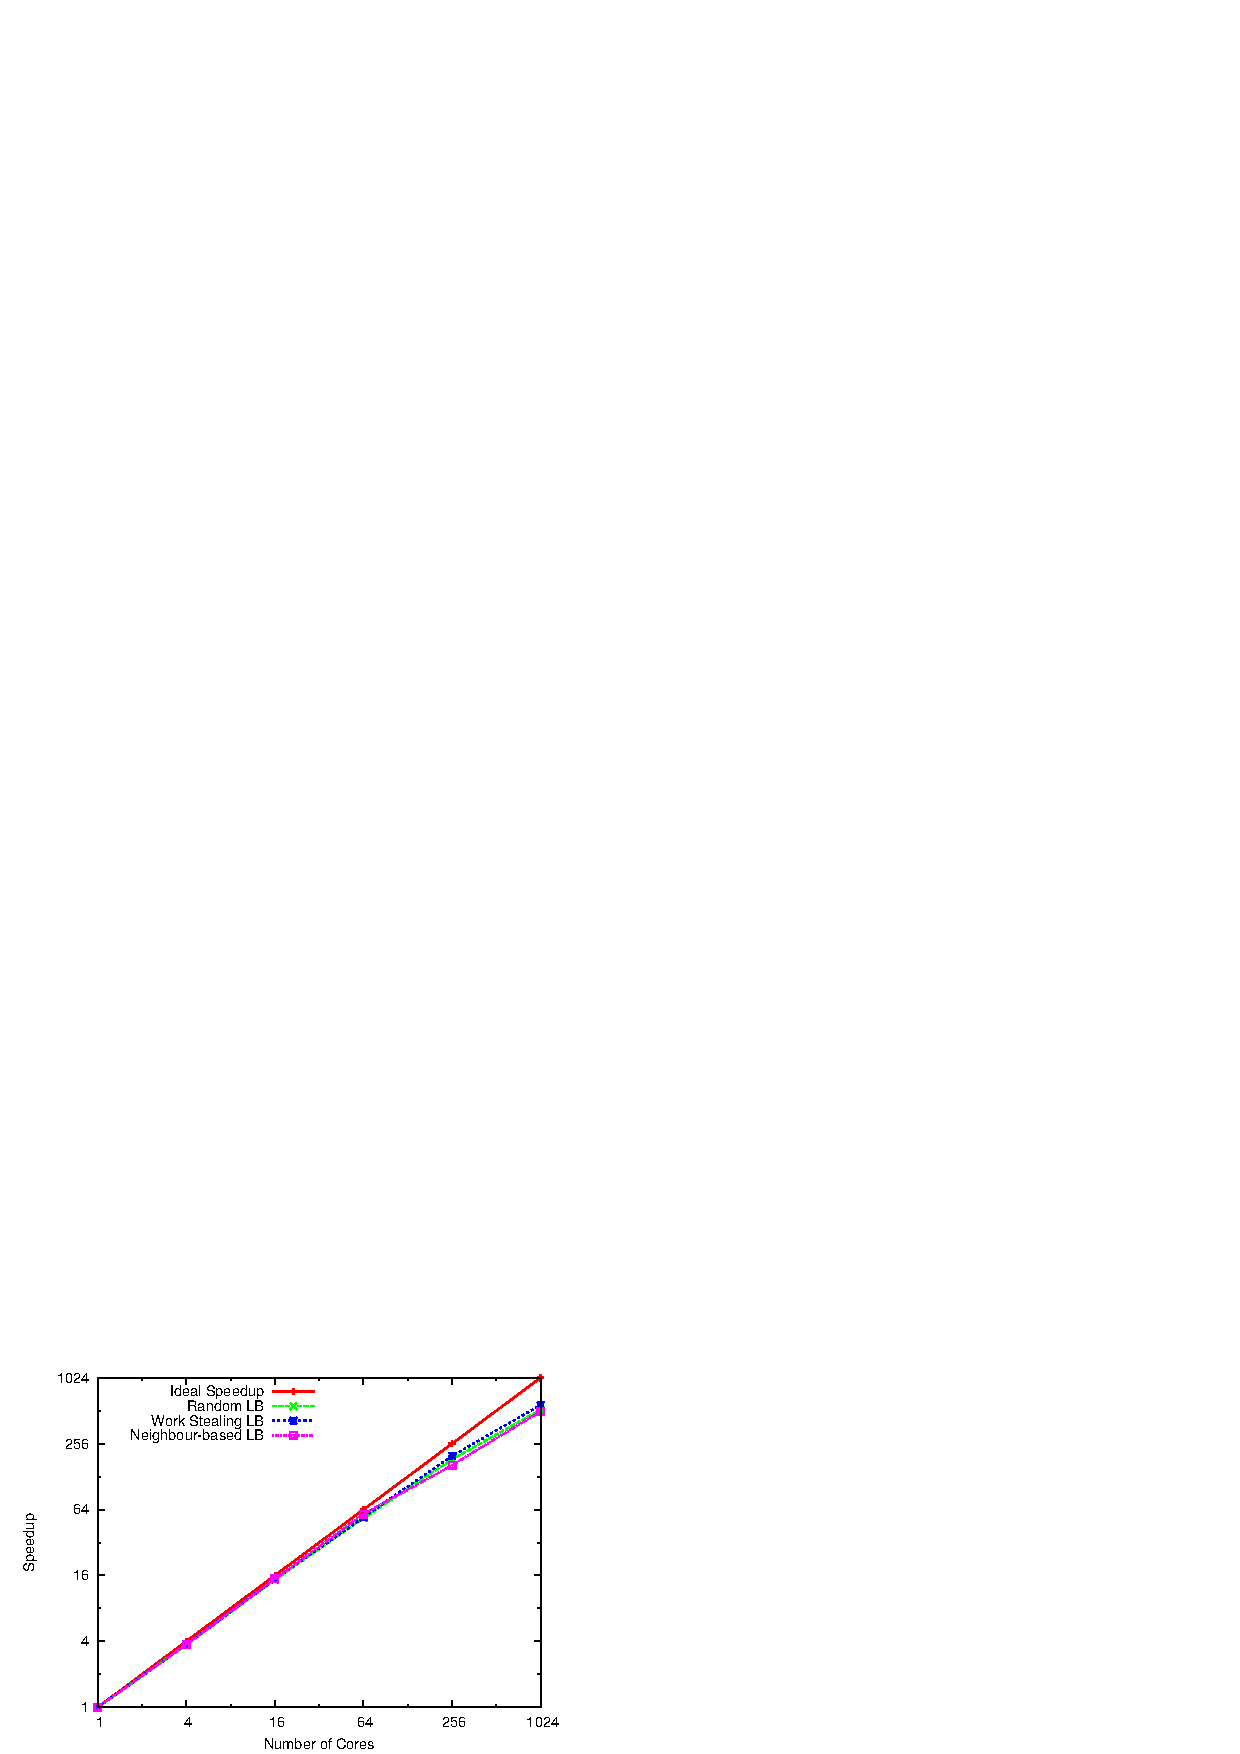
\includegraphics[width=0.9\columnwidth]{plots/3schemes.pdf}

\caption{Effect of load balancing strategy}
\label{3schemes}
\vspace{-0.2in}
\end{figure}
 

\label{grainsize}

\begin{figure*}[ht]
\centering
\subfigure[Depth 8]{
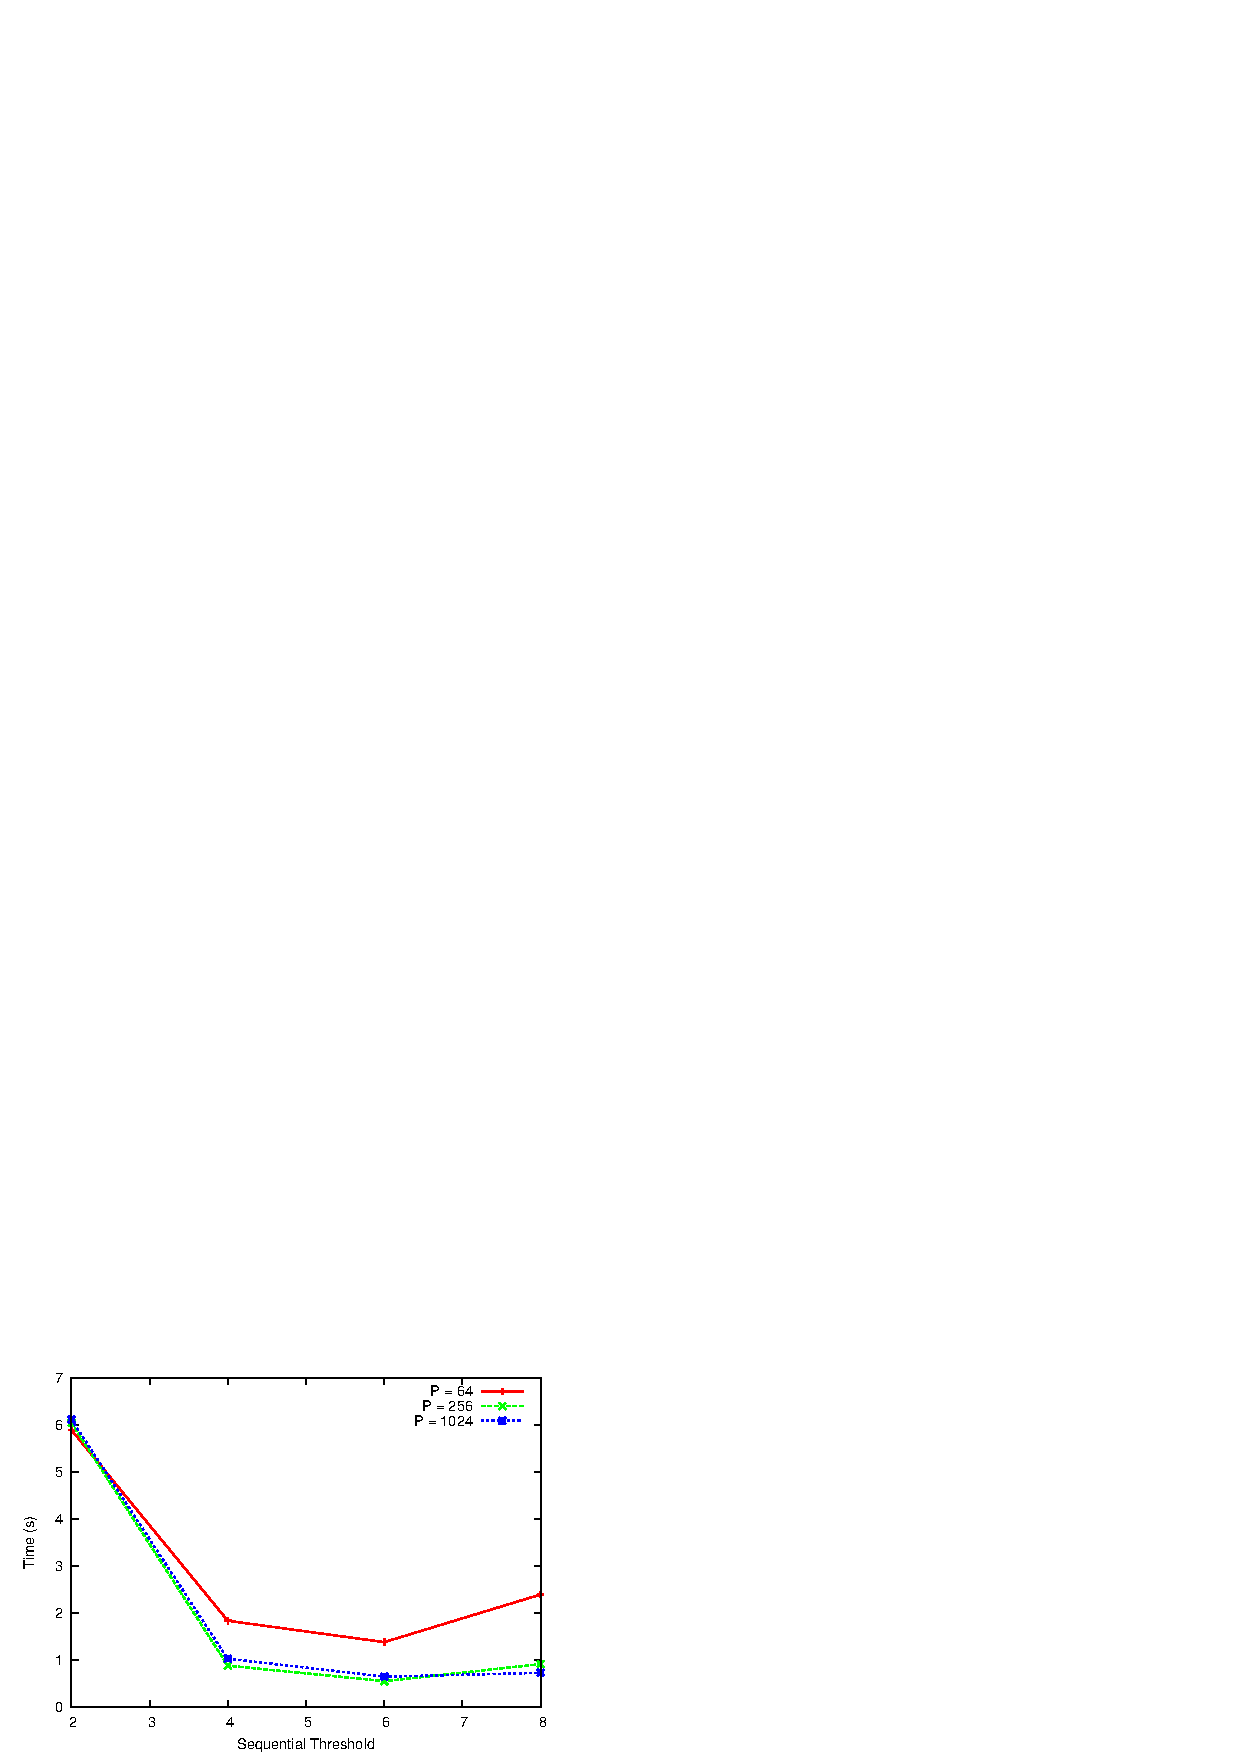
\includegraphics[width=2.1in]{plots/dep8.pdf}
\label{dep8}
} 
\subfigure[Depth 10]{
\includegraphics[width=2.1in]{plots/dep10.pdf}
\label{dep10}
} 
\subfigure[Depth 12]{
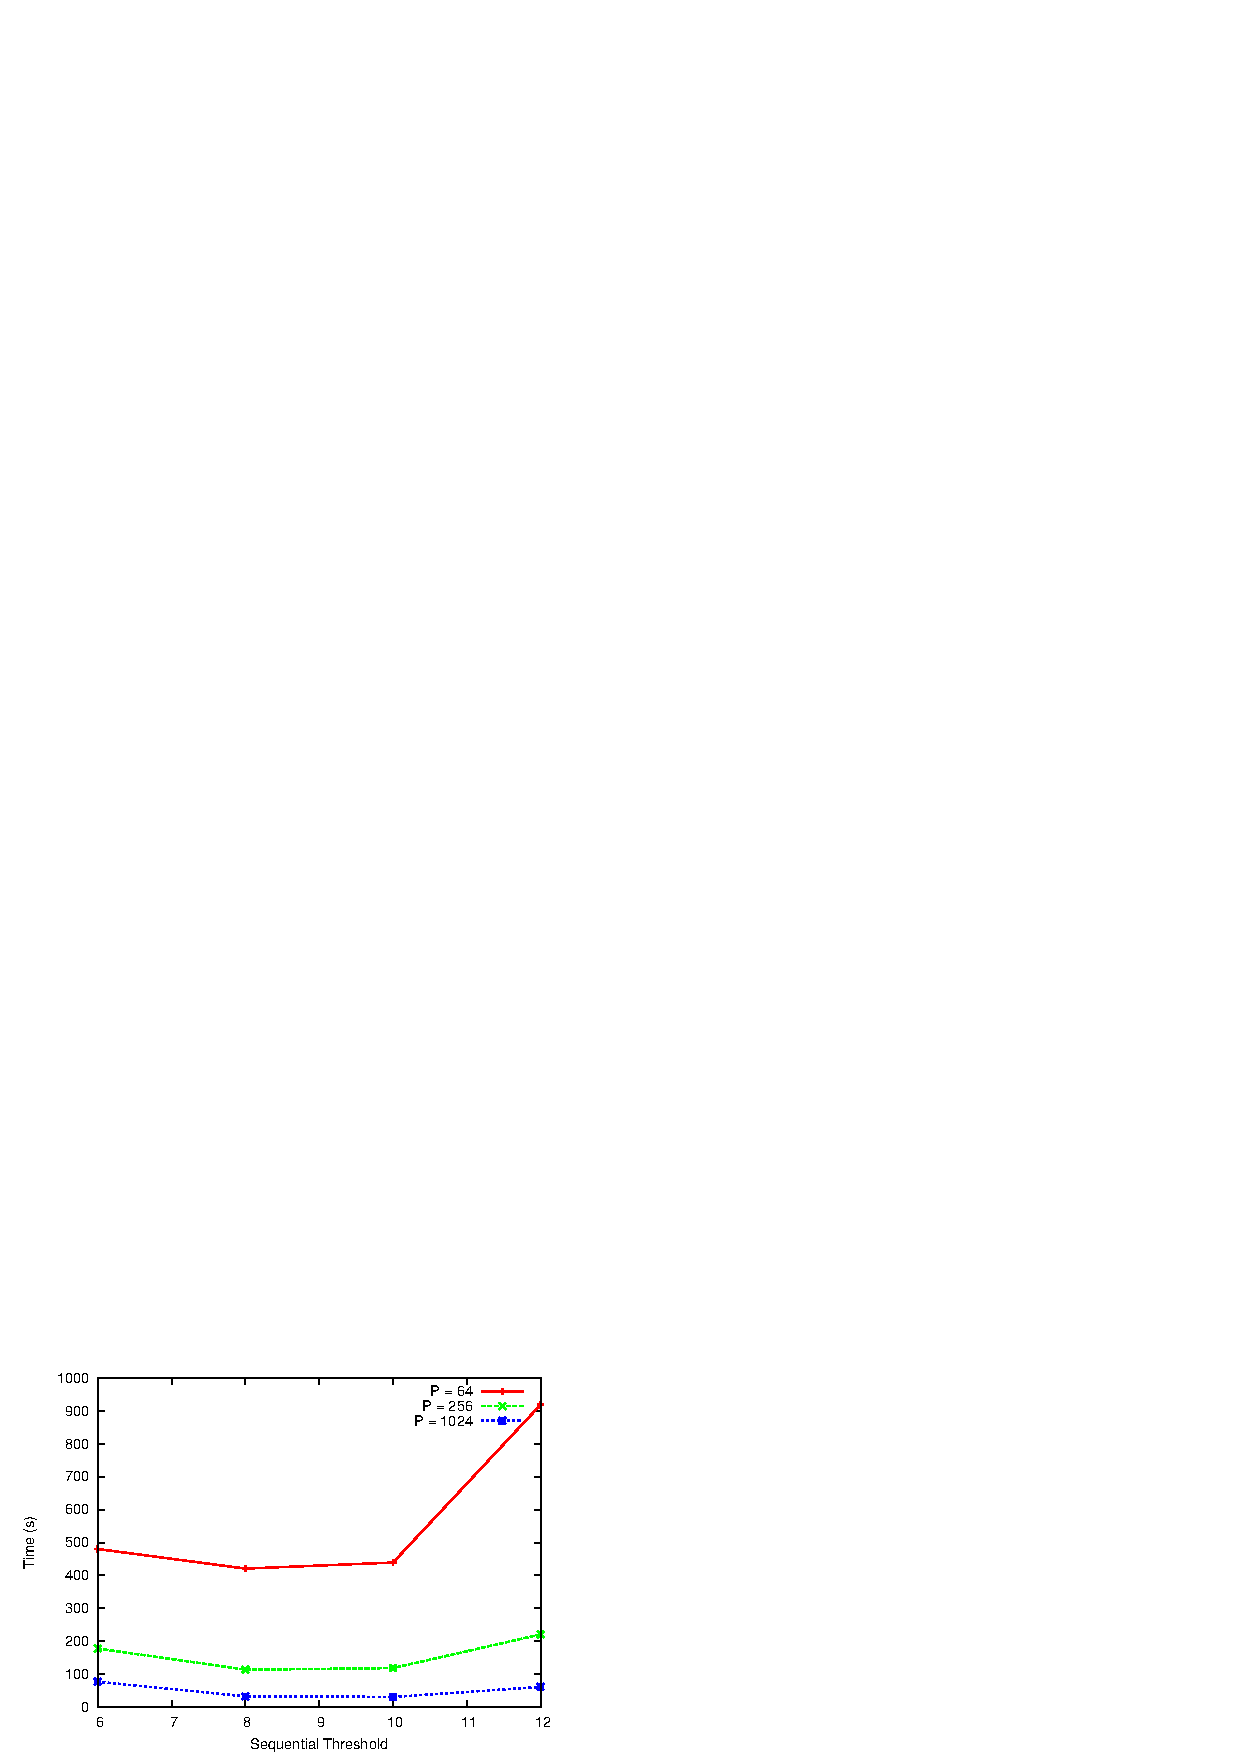
\includegraphics[width=2.1in]{plots/dep12.pdf}
\label{dep12}
} 
\caption{Grainsize Control for different problem sizes. Sequential threshold denotes the depth in the search tree after which the remainder of the task (game tree search) is performed sequentially. Grain size = max game tree depth - sequential threshold.}
%\vspace{-0.1in}
\label{fig:dep}
\vspace{-0.2in}
\end{figure*}
%


In our experiments, the sequential threshold is clearly related to the size of the
problem --- the depth of the search tree.  The optimal sequential threshold is $2-4$ less than the problem depth.  Since the depth of all solutions is
the same for each problem instance, this means that the number of levels that
should be searched sequentially (that is, optimal grain size) is fairly consistent across problem sizes.  We
noted that the number of solutions found---in other words, the size of the
information sets---is typically fairly large with respect to the total number
of nodes expanded.  (We estimate that it was often $30-40\%$).  This high
density of solutions limits the variability that can be present in the amount
of work to be done at the nodes representing the last few levels of the tree.
This means that the best grainsize is also likely to be fairly predictable,
which is encouraging.  

\subsubsection{Effect of Problem Size}


We next study the variation in the efficiency of the parallelization of the
algorithm as size of the problem increases.  Here, we varied the number
of plies in the test instance from 8 to 12. We used the work stealing
load-balancing strategy.  
\begin{figure}[ht] 
\centering
\begin{minipage}{0.7\linewidth}
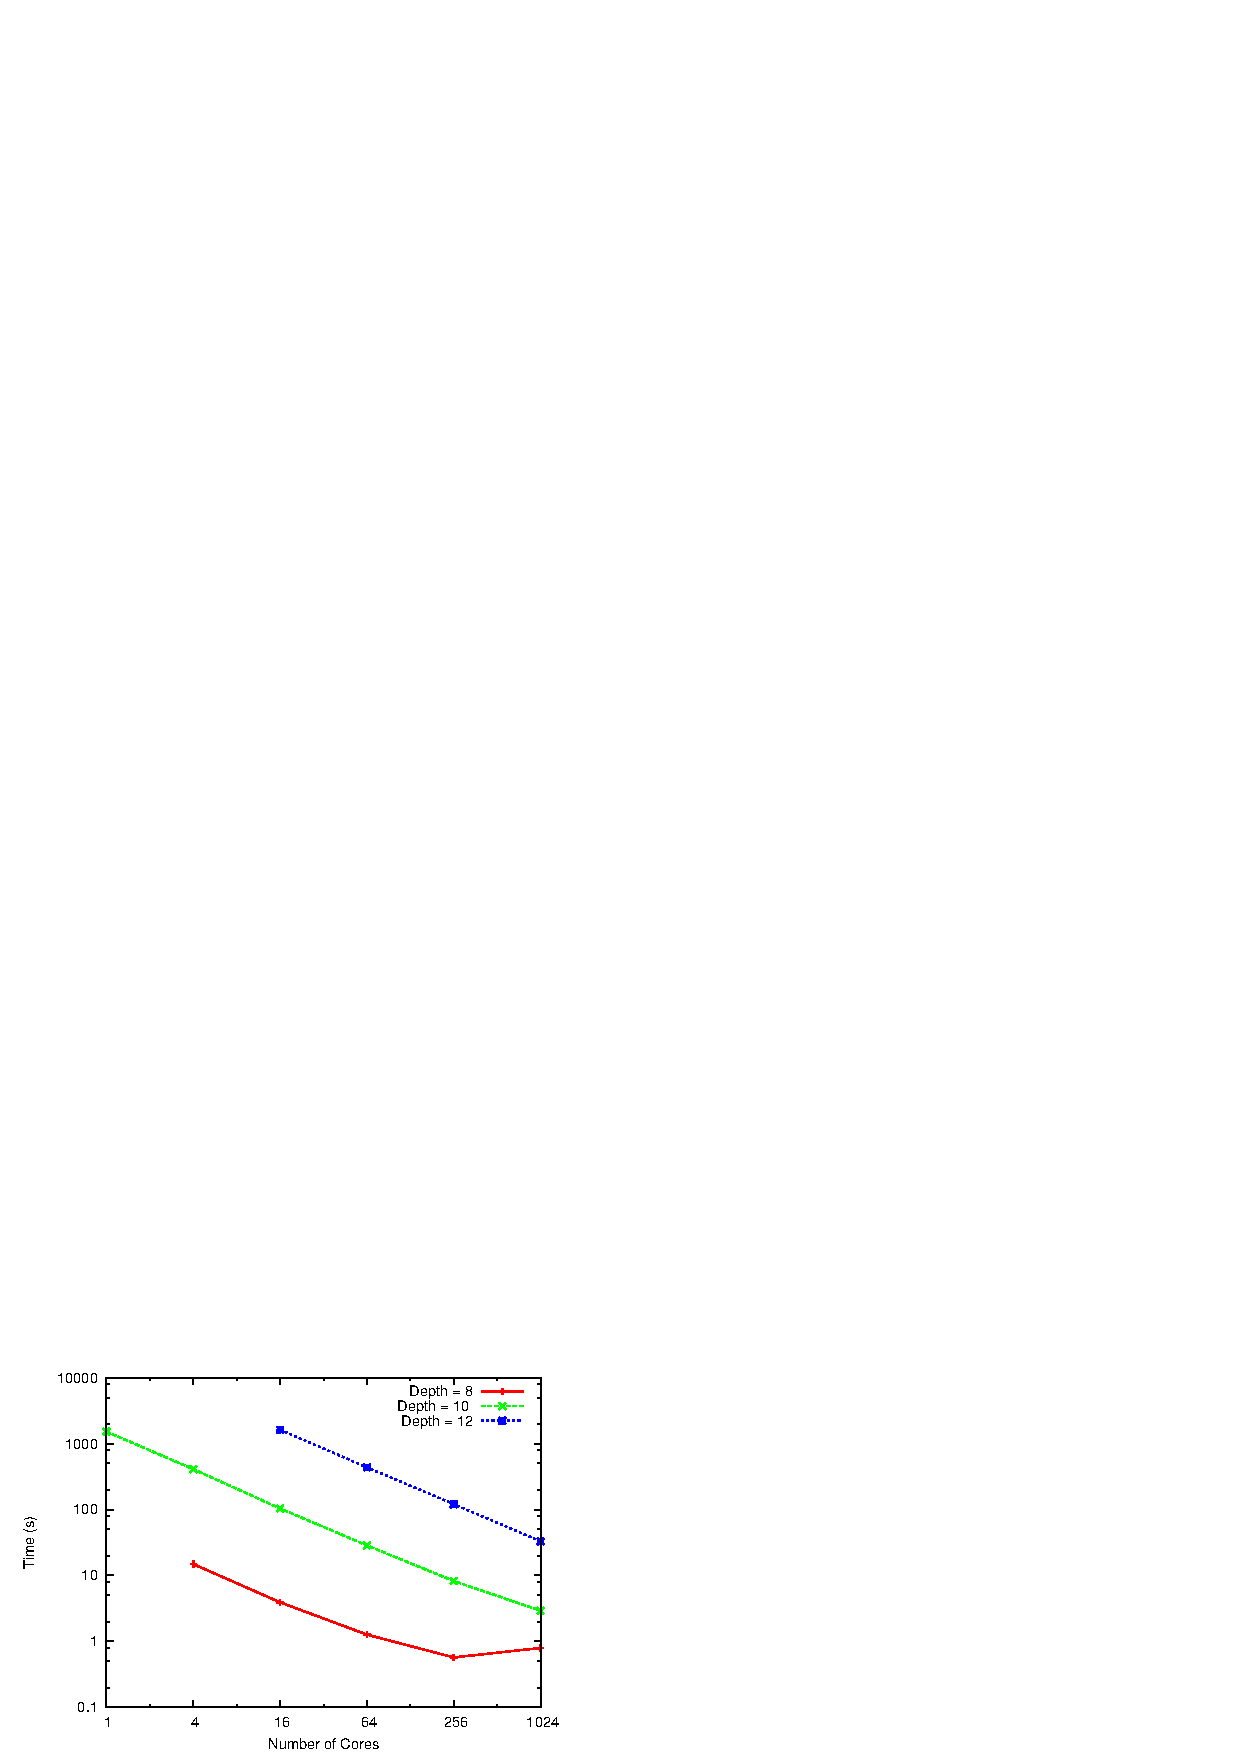
\includegraphics[width=\columnwidth]{plots/3depths.pdf}
\end{minipage}
\centering
\begin{minipage}{0.7\linewidth}
\includegraphics[width=\columnwidth]{plots/3depthspe.pdf}
\end{minipage}
\caption{(Top) Execution time for three different sizes of problem as the number of cores used increases.
(Bottom) Parallel Efficiency (wrt to 16 cores) vs number of cores, to help see the effect of problem size and iso-efficiency}
\label{3depths}
\vspace{-0.3in}
\end{figure}
The results are shown in Figure~\ref{3depths}.  In the easiest case (depth 8),
there is not enough additional parallel work to justify the jump from 256 to
1,024 processors, and performance actually degrades.  Aside from this anomaly,
however, we see consistent speedups as we increase the number of processors. 
The plot on the bottom helps to illustrate the effect of problem size on parallel efficiency (defined as Speedup/P) and helps understand the iso-efficiency of the problem. Iso-efficiency~\cite{b:grama-isoefficiency} means how should the problem size be increased with increasing number of processors to maintain same level of parallel efficiency. As the size of the problem increases, the amount of parallelizable work available also increases, and hence parallel efficiency is higher for larger problem sizes and constant number of processors (Figure~\ref{3depths} bottom). As the number of processors increases, parallel efficiency decreases for constant problem size. Figure~\ref{3depths} suggests that in parallel information set generation, to maintain constant parallel efficiency, problem size (search depth) should be roughly increased by two when the number of processor in increased by 4 times.

\begin{table}[ht]
\caption{Running times in seconds and speedups (after $|$), to find full
information set of size 764,209 at position 10 of Virgil-David 1969. Optimal
grainsize (G) for each number of cores (PE) is shown in bold.}


\centering
%\begin{tabular}{rrrrr}
\begin{tabular}{ccccc}
PE/G & 2 & 4 & 6 & 8 \\
1 & {\bf 177$|$1} & 178$|$0.99 & 1844$|$0.96 & 493$|$0.36 \\
4 & 71$|$2.48 & 53$|$3.34 & {\bf 48$|$3.63} & 75$|$2.35 \\
16 & 34$|$5.19 & 19 $|$9.27& {\bf 12$|$13.8} & 16$|$10.7 \\
64 & 24 $|$7.25 & 7 $|$23.6& {\bf 3.7$|$47.39} & 4.1$|$43.1 \\
256 & 24 $|$ 7.1& 4.4 $|$40.1 & 1.2 $|$145& {\bf 1.0$|$172} \\
1024 & 26 $|$6.61 & 3.8 $|$46.5& 0.64 $|$276& {\bf 0.40$|$443}
\end{tabular}

\label{tab:prob4}
\vspace{-0.1in}
\end{table}

\begin{table}[th]
\caption{Running times, in seconds and speedups (after $|$), to find full
information set of size 5,099,257 at position 10 of Game 6 Kbot-Darkboard 2006.
Optimal grainsize for each number of cores is shown in bold.}
\centering
%\begin{tabular}{rrrrr}
\begin{tabular}{ccccc}
PE/G & 2 & 4 & 6 & 8 \\
1 & 617$|$1 & {\bf 612$|$1} & 650$|$0.95 & 3312$|$0.19 \\
4 & 213$|$2.89 & 170$|$3.63 & {\bf 158$|$3.89} & 367$|$1.68 \\
16 & 83$|$7.41 & 49$|$12.4 & {\bf 40$|$15.1} & 64$|$9.57 \\
64 & 54$|$11.3 & 19$|$32.3 & {\bf 11$|$52.9} & 14.9$|$41.4 \\
256 & 54$|$11.3 & 9.8$|$62.9 & 3.5$|$172 & {\bf 3.5$|$174} \\
1024 & 58$|$10.6 & 5.5$|$111 & 1.3$|$464 & {\bf 1.2$|$536} \\
\end{tabular}

\label{tab:prob5}
\vspace{-0.1in}
\end{table}

\subsection{Real Game Instance}
%\begin{figure}[ht]
% \centering \includegraphics[viewport= 280 200 300 550, scale=0.35]{images/KriegspielProblem4.pdf} %
%
%\caption{Kriegspiel position from Virgil-David 1969 with information set size
%764,209.}
%
%\label{prob4} 
%\vspace{-0.2in}
%\end{figure}
%
%\begin{figure}[ht]
% \centering \includegraphics[viewport= 280 200 300 550, scale=0.35]{images/KriegspielProblem5.pdf} %
%
%\caption{Kriegspiel position from Game 6 of Kbot-Darkboard at the 2006 Computer
%Chess championship.  Information set size is 5,099,257.}
%
%\label{prob5} 
%\vspace{-0.2in}
%\end{figure}

We also evaluated our information set generation routine on 40 positions from
actual Kriegspiel games, including human vs. human and computer vs. computer
instances.  Many of these were trivial to solve in a few seconds or less on a
desktop computer.  For these experiments, we used the Ranger supercomputer
at TACC~\cite{ranger}. Ranger has 16-way SMP nodes containing AMD Opteron
processors. The nodes are interconnected using Infiniband technology in a
fully-CLOS topology providing a 1GBps point-to-point bandwidth. We used {\sc Charm++}'s \texttt{net-ibverbs} machine layer build and $-O3$ optimization for these experiments.

The running times and speedups for two of the more challenging instances are shown in Tables~\ref{tab:prob4}--\ref{tab:prob5}.   These tables
show the results for runs on one to $1,024$ cores.  Each column corresponds to
a different sequential threshold parameter - the number of
levels of the search tree that are searched in parallel.  Up to that threshold,
each node that is generated spawns a new piece of work, which the {\sc Charm++}
runtime schedules to execute on one of the processing elements according to its
load balancing strategy.  Beyond the threshold the entire subtree is searched to
completion on a single processor, with no additional parallel overhead. 

These results confirm the observations made in Section~\ref{grainsize}. The optimal sequential threshold varies for the different numbers of cores and
the pattern is consistent across problem instances.  The optimal
sequential threshold increases as the number of cores increases.  This is expected,
because as this parameter grows, the number of distinct pieces of work
increases.  When the number of chares per processor is high, much of
the overhead of parallelization is wasted.  However, as the number of cores
increases, the work can be efficiently broken up into smaller pieces and spread to all the cores.  With more pieces of work, it becomes easier to balance
the load.



Note that both problems scale well even up to 1,024 processors.  We achieve a
speedup of $443$ in the game between humans and up to $536$ in the game between
computers.  Figure~\ref{prob4} shows the plot of the running
times on these two problems with the best grainsize for each core setting.  These plots show that the
running time continues to decrease as the number of cores increases.

\section{Comparison with previous results, Discussion}
\label{discuss}
Our results compare favorably to previous work in parallel game tree search,
shown in Table~\ref{bestspeedups}.  The previous best parallelization results
were for parallelizing alpha-beta pruning.  Ferguson and Korf achieved a
speedup of 12 on 32 cores in the game of Othello~\cite{ferguson88distributed}.
In the game of chess, Felton and Otto showed a speedup of 100 on 256
cores~\cite{felten88highly}.  This limited scalability is due to speculative
loss.  Parts of the game tree that are searched during the parallel execution
would have been pruned had the algorithm run sequentially.  This is a
fundamental limitation in alpha-beta search. 

For partially observable games, information set generation represents a
different variety of tree search that does not suffer from speculative loss.
All of the nodes that are visited in parallel also would have been visited in a
sequential run.  The key challenge for parallelizing information set generation
is load balancing: some parts of the tree will be pruned at a higher level than
others, resulting in a wide variation in cost for each subtree.  The {\sc
Charm++/ParSSSE} framework is perfectly suited to handle the load balancing
issues that this problem naturally presents.

\begin{figure}[t]
 \centering \includegraphics[scale=1]{plots/new.pdf} %
\caption{Performance results for Information Set Generation for two games of Kriegspiel, position ten}
\label{prob4} 
\end{figure}


Note also that information set generation is just one subroutine needed to
reason about partially observable games.  Once plausible game histories have
been found, an agent may simulate some sequences of moves up to previous moves
made by opponents and then recursively call the ISG procedure from the
perspective of the opponent.  This results in many parallel applications of
ISG. Furthermore, given a node in an information set, it is common for an agent
to perform forward search on that node (e.g., using MCTS).  All of these
forward search operation can be performed independently in parallel. With these
two additional levels of parallelism on top of the information set generation
problem, it is likely that the problem of playing partially observable
games could scale efficiently to millions of processors or more.
\begin{table}[ht]
\caption{Best Speedups reported for game tree applications.}
\centering
\begin{tabular}{lrrc}
{\bf Authors} & {\bf Game} & {\bf Year} & {\bf Best Speedup (cores)} \\
Ferguson \& Korf & Othello & 1988 & 12(32) \\
Felton \& Otto & Chess & 1988 & 100(256) \\
Richards \etal & Kriegspiel & 2012 & 178(256) \\
Richards \etal & Kriegspiel & 2012 & {\bf 536(1024)} \\
\end{tabular}
\label{bestspeedups}
\end{table}
\section{Related Work}
\label{Related}
An overview of the theory of imperfect information games and other basic topics
in game theory can be found in~\cite{kuhn03lectures} and~\cite{kuhn97classics}.
A technical explanation of the concept of information sets can be found
in~\cite{gilpin09algorithms}.  Koller \etal, showed that a Nash equilibrium can
be found in time that is polynomial in the number of nodes in the game
tree~\cite{koller94fast}.  In fact, they found that it took about as much time
to generate the full game tree as it did to actually solve it.  Unfortunately,
this is feasible only for small games.  In larger games where theoretically
optimal strategies cannot be computed efficiently, computer systems tend to
utilize the concept of information sets or belief states in some form or
another.  A common strategy is to estimate the value of a move by averaging the
estimated value of the associated descendant for each node in the current
information set (or a random sample from the set).  While this sort of
``averaging over clairvoyance'' {\em can} lead to very poor decisions, it is
nevertheless a reasonable strategy in some games, such as
Scrabble~\cite{sheppard02world}.

In this work, we have argued for an ISG approach to Kriegspiel, but other
authors have approached the problem differently.  Parker \etal, consider the
problem of sampling from belief states in a variety of large game trees,
including Kriegspiel~\cite{parker05game}.  They show that some performance gains
can be achieved by only approximate sampling from the belief state.  Instead of
generating the full information set, or even sampling from it, they sample from
possible positions for the current state (i.e., sampling from the belief state)
by matching only the most recent observations.  The motivation for this approach
seems to be that it would not be feasible to sample from the full information
set, because of the computational expense involved. Our experiments bear this
out-- it can indeed be expensive to produce the full information set.  For the
experiments shown in Table~\ref{speedups}, generating the full information set
took over 25 minutes on a single processor.  However, by utilizing the {\sc
Charm++/ParSSSE} search engine on a parallel machine (1,024 processors), we were
able to generate the full set in just 2.9 seconds.    

%Li gives an overview of Kriegspiel and discusses strategy from the perspective of human players~\cite{li94chess}.  He
%walks through the analysis of several actual games between two human players and discusses the inferences that each
%player can and should make at each position.  As in chess, human players are able to reason about the game at an
%abstract level; they tend to focus on a small number of critical possibilities and to emphasize the most important
%pieces and squares in each position.  Computer agents, lacking such sophistication, nevertheless have some advantages
%when it comes to brute force search strategies. Programs such Deep Blue have shown that a brute force approach to game
%tree search can be effective, even against humans with vastly superior abstract reasoning capabilities, provided that
%significant computational resources are available and wisely used~\cite{campbell02deep}.

%Russell and Wolfe have performed some analysis on Kriegspiel positions for which it possible to prove that one player
%has a forced win (that is, regardless of the configuration of the opponent's unseen pieces, the player has a sequence of
%moves that is guaranteed to produce a checkmate)~\cite{russell05efficient, wolfe07exploiting}.  The authors assume
%knowledge of the player's belief state.  They claim that under certain "aggressive" styles of play, it is uncommon for
%information sets to exceed 10,000 nodes in size.  They throw out (i.e., do not analyze) any positions that exceed this
%threshold.  

%In our experiments, we have found positions in which the size of the information set is many tens of millions.  Our goal
%is to develop strategies that are amenable to use in this more general setting.   In other words, rather than being able
%to analyze positions only at the beginning or end of the game (when the size of the information set tends to be
%smaller), we want to be able to develop a strategy that can be used in the middle of the game as well.  game). 

The information set generation approach that we have presented is certainly
also computationally expensive.  And representing a full information set (e.g.,
as a list of sequences of moves that encode a path from the start state to the
current node) would be similarly expensive in terms of storage space.  However,
we have shown that our algorithm is also highly scalable.  Furthermore,
contrary to the approach in~\cite{nance06reasoning}, our approach is readily
adaptable to sampling algorithms.  Given a sample size that matches available
memory, any single sequence of moves is readily extractable without the
computational expense of a theorem prover or SAT solver.

The effect of load balancing and computational granularity on combinatorial search problems has been studied before~\cite{sun11adaptive,WeatherAmpiSBAC10}. In this work, we addressed the parallelization of an information set generation algorithm and studied the impact of these factors applied to game tree applications. %We explored an application  which has largely been unexplored by the HPC community  

%\Section{Conclusion Future Work}
%We have shown that information set generation for Kriegspiel can be efficiently parallelized in a way that scales up to at least 1,024 processors.

%A key line of future research is to use our ISG routine as part of a full Kriegspiel play.  The ISG method itself could be updated using constraint-satisfaction techniques outlined in ~\cite{richards12information}, which improve pruning performance in the search space by incorporating information from all observations in the list at each search step, instead of performing depth-first search.   The use of ISG-based opponent modeling to improve overall decision making is described in ~\cite{richards12reasoning}. 

%determined by how well that information improves a player's decision-making capabilities.  We noted earlier that a
%common use of information sets is to estimate the value of a move by averaging the estimated value of the associated
%descendant for each node in the current information set (or a random sample from the set).  This kind of strategy can be
%applied naively using a belief state sampling algorithm (i.e., an algorithm that samples from the distribution of
%possible worlds in the current state without respect to the overall history of moves).  However, it has been shown that
%significant improvement in play can be achieved by estimating the value of future moves from the perspective of the
%opponent, based on the knowledge that the opponent would have had at prior positions in the move
%history~\cite{richards07opponent}.  Such a strategy would require the use of an information set generation algorithm of the
%kind that we have described here.\footnote{This work is underway.}

%Ideally, we would run our algorithm on some deeper instances from real Kriegspiel games.  We are not aware of a
%repository of such games.  Unfortunately, notation for Kriegspiel is not standardized and there are several minor
%variations in rules (i.e., with respect to the nature of referee announcements) that are unlikely to significantly to
%impact the computability and scalability results but which nevertheless make it difficult to write an input reader that
%converts the transcript of a game into a sequence of moves readable by our algorithm.  An alternative would be to play
%some games ourselves.  Currently, the manual encoding of games is not difficult but is tedious.  Still, it would be nice
%to have some games that go on for 40 or 50 moves and have positions where the information sets are of moderate size (on
%the order of a few hundred thousand to a few million).

%The information set generation algorithm that we have implemented here is the most straightforward one and is alluded to
%in~\cite{parker05game} and~\cite{russell05efficient}.  It is analogous to the ``expand-at-the-tip'' strategy for the
%Hamiltonian Circuit problem.  An alternative information set generation algorithm is described
%in~\cite{richards09information} (but not implemented in parallel) and could potentially improve the search efficiency
%greatly by exploiting variable ordering.  This would be analogous to the disconnected edge-pairs\footnote{This is what we
%referred to as ``algorithm 2'' in class.} heuristic for the Hamiltonian Circuit problem.  Rather than search from the
%root node going forward, this algorithm would seek opportunities for pruning based on the propagation of logical
%consequences from each move both forward and backward in time.  This, incidentally, is more consistent with the way
%human players would analyze the game.  For example, if a player's proposed bishop move is rejected and the bishop is
%sufficiently removed from its own king, then the player may infer that one of his opponent's pieces is along that
%rejected path.  At least one of those spaces must have been the destination of a prior move by the opponent.  If a
%recent move by that bishop crossed the same path, then that would be hard evidence that those squares were empty at the
%time.  And therefore, the arrival of the opponent's piece must have been between the previous (successful) bishop move
%and the current (unsuccessful) bishop move.  To implement this algorithm, we envision the use of planning graph type
%data structures~\cite{blum97fast}.  Planning graphs have a sequence of alternating levels of state constraints and
%action constraints.  State constraints would be of the form $at(bishop,d4) \vee at(bishop,e6)$ or $!occupied(e4)$.
%Action constraints would be of the form $move(knight,a4,c5) \vee move(knight,e6)$.  At a minimum, each level would
%require a data structure with a bit for each possible action/state.  Propagating the constraints would require much of
%the same machinery used in STRIPS-like planning algorithms~\cite{chen05solving}, and one of the many knobs that would
%need to be tuned would be the depth of the propagation for each constraint.  (Should the consequences of a known action
%or non-action be propagated one move into the future and one move into the past?  More?  Less?)  Additionally, there
%would be a significant and interesting tradeoff in the effectiveness of pruning and the size of the data
%structures that would have to be encoded in each chare.  The best algorithm might be a hybrid strategy that does forward
%propagation from the root at the parallel level and constraint propagation at the sequential level.\footnote{This work
%is also in progress.}
%
%There are certainly several places where the efficiency of the details of each node expansion could be improved.  Many
%of these would reduce the overall running time but would not necessarily be interesting from the standpoint of
%evaluating the efficiency and iso-efficiency of parallelization.  For example, in checking to see if a position leaves a
%player in check, we currently utilize existing helper functions that generate possible moves for the opponent.  It would
%be possible to write a more specialized function that focuses only on the position of the king in question and looks
%only at the squares along its rank, file, diagonals, and knight-edges for threats.  There are also some memory
%allocation issues that could be improved. 

\section{Conclusion and Future Work}
In this paper, we showed that information set generation for Kriegspiel can be efficiently
parallelized.  Through extensive experimentation, we demonstrated that the choice of a suitable load balancing strategy and optimal grain size control is crucial to achieve good scalability for parallel ISG. The opportunities for parallelism increase as the problem size
increases.  Our algorithm has performed well on problems with information sets
with as many as 65 million nodes --- much larger than any other treatment of the
problem that we are aware of.  

Since the algorithm can be efficiently
parallelized, it would be reasonable to explore using it in a full Kriegspiel
player.  It remains to be seen whether these scalability properties hold over a
wide variety of playing styles and problem instances.  We suspect that fruitful
research remains with respect to alternative algorithms that implement variable
ordering heuristics.


%\Section{Appendix A}
%The purpose of this figure is simply to help visualize the concept of information sets in game trees.  The tree for
%Kriegspiel is very difficult to visualize/depict (even an interesting part of the tree).  Figure~\ref{fulltree} shows
%the full game tree for a simple variant of Poker known as Kuhn Poker, which we hope will serve to at least make the
%concept clear, even if the Poker game itself is not immediately relevant.  There are three cards: a king, a queen, and a
%jack.  The dealer deals one card to each of two players.  Each player antes one unit, and there is one simple round of
%betting, in which the size of the pot may be doubled.  Left branches denote check/fold; right branches denote bet/call.
%For this zero-sum game, terminal nodes are labeled with payoffs to player 1, whose decision points are shown in
%triangles.  Connections between nodes in the same information set are shown with dotted lines.  The top level shows
%three different information sets for the first player, one for each possible card that could be dealt to him.  There are
%two nodes in each set, because no matter what the deal is, there are two possibilities for the card that the other
%player holds.  The leftmost information set on the bottom level corresponds to player 1's observation that he was dealt
%a king and checked, and then the opponent wagered.  The second player has six information sets as well, but they are all
%at the same level of the tree.  Like the first player, the second player has a separate information set for each
%possible card that he could be dealt.  And the two nodes in each set are there because there are two possibilities for
%the opponent card.  The second player also gets to know whether the first player checked of bet, and that is why there
%are twice as many information sets.
%
%\begin{figure}
%\scalebox{.72}{
%\begin{tikzpicture}
%  [chance/.style={circle,draw=blue!50,fill=blue!20,thick,minimum size = 10mm},
%   terminal/.style={rectangle,draw=black!50,fill=black!20,thick, minimum size = 7mm},
%   maxer/.style={shape=regular polygon, regular polygon sides=3,draw=red!50,fill=red!30,thick,minimum size = 10mm,inner sep = 0pt},
%   miner/.style={shape=diamond,draw=green!50,fill=green!30,thick,minimum size = 10mm, inner sep = 0pt},
%   edge from parent/.style={red,thick,draw}, 
%   parent anchor=south,child anchor=north,
%   level 1/.style={sibling distance=4cm,level distance=1.4cm,
%       		growth parent anchor=south},
%   level 2/.style={sibling distance=2cm},
%   level 3/.style={sibling distance=1cm},
%   level 4/.style={sibling distance=1.0cm}]
%		\node  [chance] {}
%		    child {node (M1) [maxer] {\scalebox{.75}{K}}
%			child {node (M11) [miner] {\scalebox{.75}{Q-}}
%				child {node (M111) [terminal] {1}}
%				child {node (M112) [maxer] {\scalebox{.75}{K+}}
%					child {node (M1121) [terminal] {-1}}
%					child {node (M1122) [terminal] {2}}}
%			}
%			child {node (M12) [miner] {\scalebox{.75}{Q+}}
%				child {node (M121) [terminal] {1}}
%				child {node (M122) [terminal] {2}}
%			}
%		    }
%		    child {node (M2) [maxer] {\scalebox{.75}{J}}
%			child {node (M21) [miner] {\scalebox{.75}{Q-}}
%				child {node (M211) [terminal] {-1}}
%				child {node (M212) [maxer] {\scalebox{.75}{J+}}
%					child {node (M2121) [terminal] {-1}}
%					child {node (M2122) [terminal] {-2}}}
%			}
%			child {node (M22) [miner] {\scalebox{.75}{Q+}}
%				child {node (M221) [terminal] {1}}
%				child {node (M222) [terminal] {-2}}
%			}
%		    }
%		    child {node (M3) [maxer] {\scalebox{.75}{K}}
%			child {node (M31) [miner] {\scalebox{.75}{J-}}
%				child {node (M311) [terminal] {1}}
%				child {node (M312) [maxer] {\scalebox{.75}{K+}}
%					child {node (M3121) [terminal] {-1}}
%					child {node (M3122) [terminal] {2}}}
%			}
%			child {node (M32) [miner] {\scalebox{.75}{J+}}
%				child {node (M321) [terminal] {1}}
%				child {node (M322) [terminal] {2}}
%			}
%		    }
%		    child {node (M4) [maxer] {\scalebox{.75}{Q}}
%			child {node (M41) [miner] {\scalebox{.75}{J-}}
%				child {node (M411) [terminal] {1}}
%				child {node (M412) [maxer] {\scalebox{.75}{Q+}}
%					child {node (M4121) [terminal] {-1}}
%					child {node (M4122) [terminal] {2}}}
%			}
%			child {node (M42) [miner] {\scalebox{.75}{J+}}
%				child {node (M421) [terminal] {1}}
%				child {node (M422) [terminal] {2}}
%			}
%		    }
%		    child {node (M5) [maxer] {\scalebox{.75}{J}}
%			child {node (M51) [miner] {\scalebox{.75}{K-}}
%				child {node (M511) [terminal] {-1}}
%				child {node (M512) [maxer] {\scalebox{.75}{J+}}
%					child {node (M5121) [terminal] {-1}}
%					child {node (M5122) [terminal] {-2}}}
%			}
%			child {node (M52) [miner] {\scalebox{.75}{K+}}
%				child {node (M521) [terminal] {1}}
%				child {node (M522) [terminal] {-2}}
%			}
%		    }
%		    child {node (M6) [maxer] {\scalebox{.75}{Q}}
%			child {node (M61) [miner] {\scalebox{.75}{K-}}
%				child {node (M611) [terminal] {-1}}
%				child {node (M612) [maxer] {\scalebox{.75}{Q+}}
%					child {node (M6121) [terminal] {-1}}
%					child {node (M6122) [terminal] {-2}}}
%			}
%			child {node (M62) [miner] {\scalebox{.75}{K+}}
%				child {node (M621) [terminal] {1}}
%				child {node (M622) [terminal] {-2}}
%			}
%		    };
%		\draw  (M1.north) to [dashed,black,out=15,in=165] (M3.north);
%		\draw  (M2.north) to [dashed,black,out=15,in=165] (M5.north);
%		\draw  (M4.north) to [dashed,black,out=15,in=165] (M6.north);
%		\draw  (M112.north) to [dashed,black,out=15,in=165] (M312.north);
%		\draw  (M212.north) to [dashed,black,out=15,in=165] (M512.north);
%		\draw  (M412.north) to [dashed,black,out=15,in=165] (M612.north);
%		\draw  (M11.north) to [dashed,black,out=15,in=165] (M21.north);
%		\draw  (M12.north) to [dashed,black,out=15,in=165] (M22.north);
%		\draw  (M31.north) to [dashed,black,out=15,in=165] (M41.north);
%		\draw  (M32.north) to [dashed,black,out=15,in=165] (M42.north);
%		\draw  (M51.north) to [dashed,black,out=15,in=165] (M61.north);
%		\draw  (M52.north) to [dashed,black,out=15,in=165] (M62.north);
%\end{tikzpicture}
%} %scalebox
%\caption{}
%\label{fulltree}
%\end{figure}




%\nocite{*}
%\nocite{richards09information}
%\nocite{russell05efficient}
%\nocite{kuhn03lectures}
%\nocite{kuhn97classics}
%\nocite{parker05sampling}
%\nocite{nance06reasoning}
%\nocite{li94chess}

%\begin{thebibliography}{99}
%\end{thebibliography}


%\begin{figure}

%\Section{Appendix B}
%Verbose output from the information set generation algorithm.  The listing shows possible sequences of moves that are
%consistent with the black's observations after ten plies.  The resulting position after each consistent sequence of
%moves is shown below.  Based on these results, black can know with certainty the location of white's pawn at d6 and
%white's bishop at g5.
%
%\begin{verbatim}
%1. Pa2:a4 Pa7:a5 2. Pd2:d4 Pb7:b6 3. Bc1:g5 Pc7:c5 4. Pd4:d5 Nb8:a6 5. Pd5:d6 Pf7:f6 
%
%**********************************************
%R - B Q K B N R 
%- - - P P - P P 
%N P - p - P - - 
%P - P - - - b - 
%p - - - - - - - 
%- - - - - - - - 
%- p p - p p p p 
%r n - q k b n r 
%**********************************************
%1. Pd2:d3 Pa7:a5 2. Bc1:g5 Pb7:b6 3. Pd3:d4 Pc7:c5 4. Pd4:d5 Nb8:a6 5. Pd5:d6 Pf7:f6 
%
%**********************************************
%R - B Q K B N R 
%- - - P P - P P 
%N P - p - P - - 
%P - P - - - b - 
%- - - - - - - - 
%- - - - - - - - 
%p p p - p p p p 
%r n - q k b n r 
%**********************************************
%1. Pd2:d4 Pa7:a5 2. Pa2:a4 Pb7:b6 3. Bc1:g5 Pc7:c5 4. Pd4:d5 Nb8:a6 5. Pd5:d6 Pf7:f6 
%
%**********************************************
%R - B Q K B N R 
%- - - P P - P P 
%N P - p - P - - 
%P - P - - - b - 
%p - - - - - - - 
%- - - - - - - - 
%- p p - p p p p 
%r n - q k b n r 
%**********************************************
%1. Pd2:d4 Pa7:a5 2. Bc1:f4 Pb7:b6 3. Bf4:g5 Pc7:c5 4. Pd4:d5 Nb8:a6 5. Pd5:d6 Pf7:f6 
%
%**********************************************
%R - B Q K B N R 
%- - - P P - P P 
%N P - p - P - - 
%P - P - - - b - 
%- - - - - - - - 
%- - - - - - - - 
%p p p - p p p p 
%r n - q k b n r 
%**********************************************
%1. Pd2:d4 Pa7:a5 2. Bc1:g5 Pb7:b6 3. Pa2:a3 Pc7:c5 4. Pd4:d5 Nb8:a6 5. Pd5:d6 Pf7:f6 
%
%**********************************************
%R - B Q K B N R 
%- - - P P - P P 
%N P - p - P - - 
%P - P - - - b - 
%- - - - - - - - 
%p - - - - - - - 
%- p p - p p p p 
%r n - q k b n r 
%**********************************************
%1. Pd2:d4 Pa7:a5 2. Bc1:g5 Pb7:b6 3. Pa2:a4 Pc7:c5 4. Pd4:d5 Nb8:a6 5. Pd5:d6 Pf7:f6 
%
%**********************************************
%R - B Q K B N R 
%- - - P P - P P 
%N P - p - P - - 
%P - P - - - b - 
%p - - - - - - - 
%- - - - - - - - 
%- p p - p p p p 
%r n - q k b n r 
%**********************************************
%1. Pd2:d4 Pa7:a5 2. Bc1:g5 Pb7:b6 3. Pb2:b3 Pc7:c5 4. Pd4:d5 Nb8:a6 5. Pd5:d6 Pf7:f6 
%
%**********************************************
%R - B Q K B N R 
%- - - P P - P P 
%N P - p - P - - 
%P - P - - - b - 
%- - - - - - - - 
%- p - - - - - - 
%p - p - p p p p 
%r n - q k b n r 
%**********************************************
%1. Pd2:d4 Pa7:a5 2. Bc1:g5 Pb7:b6 3. Pc2:c3 Pc7:c5 4. Pd4:d5 Nb8:a6 5. Pd5:d6 Pf7:f6 
%
%**********************************************
%R - B Q K B N R 
%- - - P P - P P 
%N P - p - P - - 
%P - P - - - b - 
%- - - - - - - - 
%- - p - - - - - 
%p p - - p p p p 
%r n - q k b n r 
%**********************************************
%1. Pd2:d4 Pa7:a5 2. Bc1:g5 Pb7:b6 3. Pe2:e3 Pc7:c5 4. Pd4:d5 Nb8:a6 5. Pd5:d6 Pf7:f6 
%
%**********************************************
%R - B Q K B N R 
%- - - P P - P P 
%N P - p - P - - 
%P - P - - - b - 
%- - - - - - - - 
%- - - - p - - - 
%p p p - - p p p 
%r n - q k b n r 
%**********************************************
%1. Pd2:d4 Pa7:a5 2. Bc1:g5 Pb7:b6 3. Pe2:e4 Pc7:c5 4. Pd4:d5 Nb8:a6 5. Pd5:d6 Pf7:f6 
%
%**********************************************
%R - B Q K B N R 
%- - - P P - P P 
%N P - p - P - - 
%P - P - - - b - 
%- - - - p - - - 
%- - - - - - - - 
%p p p - - p p p 
%r n - q k b n r 
%**********************************************
%1. Pd2:d4 Pa7:a5 2. Bc1:g5 Pb7:b6 3. Pf2:f3 Pc7:c5 4. Pd4:d5 Nb8:a6 5. Pd5:d6 Pf7:f6 
%
%**********************************************
%R - B Q K B N R 
%- - - P P - P P 
%N P - p - P - - 
%P - P - - - b - 
%- - - - - - - - 
%- - - - - p - - 
%p p p - p - p p 
%r n - q k b n r 
%**********************************************
%1. Pd2:d4 Pa7:a5 2. Bc1:g5 Pb7:b6 3. Pf2:f4 Pc7:c5 4. Pd4:d5 Nb8:a6 5. Pd5:d6 Pf7:f6 
%
%**********************************************
%R - B Q K B N R 
%- - - P P - P P 
%N P - p - P - - 
%P - P - - - b - 
%- - - - - p - - 
%- - - - - - - - 
%p p p - p - p p 
%r n - q k b n r 
%**********************************************
%1. Pd2:d4 Pa7:a5 2. Bc1:g5 Pb7:b6 3. Pg2:g3 Pc7:c5 4. Pd4:d5 Nb8:a6 5. Pd5:d6 Pf7:f6 
%
%**********************************************
%R - B Q K B N R 
%- - - P P - P P 
%N P - p - P - - 
%P - P - - - b - 
%- - - - - - - - 
%- - - - - - p - 
%p p p - p p - p 
%r n - q k b n r 
%**********************************************
%1. Pd2:d4 Pa7:a5 2. Bc1:g5 Pb7:b6 3. Pg2:g4 Pc7:c5 4. Pd4:d5 Nb8:a6 5. Pd5:d6 Pf7:f6 
%
%**********************************************
%R - B Q K B N R 
%- - - P P - P P 
%N P - p - P - - 
%P - P - - - b - 
%- - - - - - p - 
%- - - - - - - - 
%p p p - p p - p 
%r n - q k b n r 
%**********************************************
%1. Pd2:d4 Pa7:a5 2. Bc1:g5 Pb7:b6 3. Ph2:h3 Pc7:c5 4. Pd4:d5 Nb8:a6 5. Pd5:d6 Pf7:f6 
%
%**********************************************
%R - B Q K B N R 
%- - - P P - P P 
%N P - p - P - - 
%P - P - - - b - 
%- - - - - - - - 
%- - - - - - - p 
%p p p - p p p - 
%r n - q k b n r 
%**********************************************
%1. Pd2:d4 Pa7:a5 2. Bc1:g5 Pb7:b6 3. Ph2:h4 Pc7:c5 4. Pd4:d5 Nb8:a6 5. Pd5:d6 Pf7:f6 
%
%**********************************************
%R - B Q K B N R 
%- - - P P - P P 
%N P - p - P - - 
%P - P - - - b - 
%- - - - - - - p 
%- - - - - - - - 
%p p p - p p p - 
%r n - q k b n r 
%**********************************************
%1. Pd2:d4 Pa7:a5 2. Bc1:g5 Pb7:b6 3. Nb1:a3 Pc7:c5 4. Pd4:d5 Nb8:a6 5. Pd5:d6 Pf7:f6 
%
%**********************************************
%R - B Q K B N R 
%- - - P P - P P 
%N P - p - P - - 
%P - P - - - b - 
%- - - - - - - - 
%n - - - - - - - 
%p p p - p p p p 
%r - - q k b n r 
%**********************************************
%1. Pd2:d4 Pa7:a5 2. Bc1:g5 Pb7:b6 3. Nb1:c3 Pc7:c5 4. Pd4:d5 Nb8:a6 5. Pd5:d6 Pf7:f6 
%
%**********************************************
%R - B Q K B N R 
%- - - P P - P P 
%N P - p - P - - 
%P - P - - - b - 
%- - - - - - - - 
%- - n - - - - - 
%p p p - p p p p 
%r - - q k b n r 
%**********************************************
%1. Pd2:d4 Pa7:a5 2. Bc1:g5 Pb7:b6 3. Nb1:d2 Pc7:c5 4. Pd4:d5 Nb8:a6 5. Pd5:d6 Pf7:f6 
%
%**********************************************
%R - B Q K B N R 
%- - - P P - P P 
%N P - p - P - - 
%P - P - - - b - 
%- - - - - - - - 
%- - - - - - - - 
%p p p n p p p p 
%r - - q k b n r 
%**********************************************
%1. Pd2:d4 Pa7:a5 2. Bc1:g5 Pb7:b6 3. Qd1:d2 Pc7:c5 4. Pd4:d5 Nb8:a6 5. Pd5:d6 Pf7:f6 
%
%**********************************************
%R - B Q K B N R 
%- - - P P - P P 
%N P - p - P - - 
%P - P - - - b - 
%- - - - - - - - 
%- - - - - - - - 
%p p p q p p p p 
%r n - - k b n r 
%**********************************************
%1. Pd2:d4 Pa7:a5 2. Bc1:g5 Pb7:b6 3. Qd1:d3 Pc7:c5 4. Pd4:d5 Nb8:a6 5. Pd5:d6 Pf7:f6 
%
%**********************************************
%R - B Q K B N R 
%- - - P P - P P 
%N P - p - P - - 
%P - P - - - b - 
%- - - - - - - - 
%- - - q - - - - 
%p p p - p p p p 
%r n - - k b n r 
%**********************************************
%1. Pd2:d4 Pa7:a5 2. Bc1:g5 Pb7:b6 3. Qd1:c1 Pc7:c5 4. Pd4:d5 Nb8:a6 5. Pd5:d6 Pf7:f6 
%
%**********************************************
%R - B Q K B N R 
%- - - P P - P P 
%N P - p - P - - 
%P - P - - - b - 
%- - - - - - - - 
%- - - - - - - - 
%p p p - p p p p 
%r n q - k b n r 
%**********************************************
%1. Pd2:d4 Pa7:a5 2. Bc1:g5 Pb7:b6 3. Ke1:d2 Pc7:c5 4. Pd4:d5 Nb8:a6 5. Pd5:d6 Pf7:f6 
%
%**********************************************
%R - B Q K B N R 
%- - - P P - P P 
%N P - p - P - - 
%P - P - - - b - 
%- - - - - - - - 
%- - - - - - - - 
%p p p k p p p p 
%r n - q - b n r 
%**********************************************
%1. Pd2:d4 Pa7:a5 2. Bc1:g5 Pb7:b6 3. Ng1:f3 Pc7:c5 4. Pd4:d5 Nb8:a6 5. Pd5:d6 Pf7:f6 
%
%**********************************************
%R - B Q K B N R 
%- - - P P - P P 
%N P - p - P - - 
%P - P - - - b - 
%- - - - - - - - 
%- - - - - n - - 
%p p p - p p p p 
%r n - q k b - r 
%**********************************************
%1. Pd2:d4 Pa7:a5 2. Bc1:g5 Pb7:b6 3. Ng1:h3 Pc7:c5 4. Pd4:d5 Nb8:a6 5. Pd5:d6 Pf7:f6 
%
%**********************************************
%R - B Q K B N R 
%- - - P P - P P 
%N P - p - P - - 
%P - P - - - b - 
%- - - - - - - - 
%- - - - - - - n 
%p p p - p p p p 
%r n - q k b - r 
%**********************************************
%Solutions founds: 25
%\end{verbatim}
%%\caption{Verbose output from example game.  Generating information sets for black after five turns by each player.
%%From this, black can infer that there is definitely a white bishop at g5 and a white pawn at d6.}
%%\label{verboseoutput}
%%\end{figure}

\bibliographystyle{IEEEtran}
\bibliography{paper,cited,group}

\end{document}
